\documentclass[12pt]{report}
\usepackage[margin=1in]{geometry} 
\usepackage[numbers,sort&compress]{natbib}
\usepackage{notoccite}
\usepackage{titlesec}
\usepackage{appendix, apptools}
\AtAppendix{%
\titleformat{\chapter}[display]{\vspace*{-30pt}\bfseries\huge}{\chaptername~\thechapter}{1em}{}
\titlespacing*{\chapter}{0pt}{0pt}{10pt}}%
\usepackage{graphicx}
\usepackage{amsmath,amssymb,amsfonts}
\usepackage{nomencl}

\makenomenclature
\linespread{2.0}
\usepackage{times}

\usepackage{caption}
\captionsetup{margin=10pt,font=sl,labelfont=bf,labelsep=period}

\makeatletter
\newcommand\appendix@chapter[1]{%
  \refstepcounter{chapter}%
  \orig@chapter*{Appendix \@Alph\c@chapter: #1}%
  \addcontentsline{toc}{chapter}{Appendix \@Alph\c@chapter: #1}%
}
\let\orig@chapter\chapter
\g@addto@macro\appendix{\let\chapter\appendix@chapter}
\makeatother

\tolerance=1
\emergencystretch=\maxdimen
\hyphenpenalty=10000
\hbadness=10000

\begin{document}
\pagenumbering{roman}
\section{Acknoledgements}

They say it takes a village to raise a child. In this case, it took a village to complete this research. 

Firstly, this entire project would not have been possible without the support from my advisor, Dr. Michelle Rosen. 

During my senior year of undergrad, Dr. Rosen invited Brandon Bunt and I to complete an independent study in Soft Robotics, and over 2 years later, here we are!
% Brandon and I were tasked with developing a \emph{backwards} robot, one that uncurled with actuation instead of the typical curling behavior like a finger. After one semester, we were able to fabricate a few robots exhibiting this backwards bending behavior and I decided to continue pursuing this research,

In the Fall 2022, Dr. Rosen hired several undergraduate research assitants: Elise Danko, Ruslana Bukalo, Erika Gregory, Sophia Xu, Randel Placino, and Claire Park were instrumental in iterating the fabrication process and experimentation procedures, and each of them were always willing and able to test out my new, wacky ideas to create this robot. 

The experimentation equiptment would not have been possible without the guidance of Michael Giglia, who taught me more than words can describe about designing robust experimentation systems and robotics.

In 2023, Dr. Rosen hired Isaiah Rivera who upgraded the electronics for pressure rig to provide more precise control. For measuring the bending behavior of the robots, it would not have been possible without the software written by Joya Debi, Isaiah Rivera, and Ani Vardanyan. 

The background research was possible through James Malin, the librarian, who showed me how to navigate the world of academic research. 

I would not have gotten through these last 2 years at Cooper without the support from the Deans, Lisa Shay and Barry Shoop. 

I would like to thank the person who found me at the end of each day around 11:30pm, who wiped my chalkboard, cleaned my lab bench, swept the floors, and took out the trash in the lab each day. Knowing you would always be there with a smile at the end of each long day made it all possible. 

I would like to thank my friends, each one of you made this possible for me. Thank you Douglas Thornhill, Catherine Van West, Jacob Koziej, Jonathan Lu, Ridwan Hussain, and Alice Cruz. 

Finally, I would like to thank my parents and grandparents, who always believed I could succeeed in STEM and who made it possible for me to live out my dreams of living in New York City and studying robotics. 
\section*{Abstract}

Soft robots, specifically soft pneumatic actuators, generate bending motion through asymmetrically constraining the deformation of soft materials. Typically, actuators are fabricated with multiple chambers or soft materials to achieve multi-directional bending within one robot. However, the increased complexity and hardware required to control these robots limit mass production and applicability for the robot. This work presents a circular soft pneumatic actuator capable of bi-directional bending with a single chamber made from a single soft material and a positive pressure source. This work documents the development and characterization of this robot and its novel method of achieving bending behavior. We include the design, iterations of the fabrication process, and the construction of the pressurization equipment. For characterization, we define an analytical model for bending angle with increasing pressure and compare it to experimental results for actuators made from four soft materials. Additionally, we measure the blocked force on the end of an actuator and present results of grasping applications for a single circular actuator. 


\tableofcontents
\listoffigures

\nomenclature{$\psi_0$}{Initial bending angle}
\nomenclature{$\psi$}{Bending angle}
\nomenclature{$r_0$}{Initial bending radius}
\nomenclature{$r$}{Bending radius}
\nomenclature{$l_0$}{Length of inextensible layer}
\nomenclature{$P$}{Input pressure}
\nomenclature{$\lambda_1$}{Axial stretch ratio}
\nomenclature{$\lambda_2$}{Circumferential stretch ratio}
\nomenclature{$\lambda_3$}{Radial stretch ratio}
\nomenclature{$\beta$}{Coordiante in base layer away from inextensible layer}
\nomenclature{$\varphi$}{Swept angle of semi circular region}
\nomenclature{$\tau$}{Coordinate in the $\varphi$ direction}
\nomenclature{$b$}{Thickness of base region}
\nomenclature{$a_0$}{Undeformed radius of semi-circular region}
\nomenclature{$t_0$}{Undeformed thickness of semi-circular region}
\nomenclature{$a$}{Deformed radius of semi-circular region}
\nomenclature{$t$}{Deformed thickness of semi-circular region}
\nomenclature{$q$}{Vertical offset of $a$ in deformed cross-section}
\nomenclature{$\varphi_m$}{Maximum $\varphi$ for deformed cross-section}
\nomenclature{$\varphi'$}{Scaled $\varphi$ for deformed cross-section}
\nomenclature{$\tau'$}{Scaled $\tau$ for deformed cross-section}
\nomenclature{$\lambda_\beta$}{Axial stretch ratio for base region}
\nomenclature{$\lambda_{\varphi,\tau}$}{Axial stretch ratio for semi-circular region}
\nomenclature{$\lambda_c$}{Circumferential stretch ratio}
\nomenclature{$\lambda_r$}{Radial stretch ratio}
\nomenclature{$k_t$}{Experimentally deturmined scale factor for thickness}
\nomenclature{$A_0$}{Area of cross-section}
\nomenclature{$W$}{Strain-energy density}
\nomenclature{$\mu_p$, $\alpha_p$}{Coefficients for Ogden material model, $p$ = 1,2,3}
\nomenclature{$\mu$}{Coefficient for Neohookean material model}
\nomenclature{$\sigma$}{Cauchy stress}
\nomenclature{$p$}{Lagrange multipler for Cauchy stress}
\nomenclature{$\sigma_1$}{Axial stress}
\nomenclature{$\sigma_2$}{Circumferential stress}
\nomenclature{$\sigma_3$}{Radial stress}
\nomenclature{$M_P$}{Moment from pressure}
\nomenclature{$M_\sigma$}{Moment from axial stress}
\nomenclature{$O$}{Neutral axis}
\nomenclature{$\sigma_\beta$}{Axial stress in base region}
\nomenclature{$\sigma_{\varphi,\tau}$}{Axial stress in deformed semi-circular region}
\nomenclature{$k_p$}{Experimentally deturmined scale factor for pressure}
\nomenclature{$\kappa$}{Curvature}
\nomenclature{$x_1$, $x_2$, $x_3$, $y_1$, $y_2$, $y_3$}{Coordinates used to calculate curvature}
\nomenclature{$F$}{Blocked Force}
\nomenclature{$e$}{Eccentricity}
\nomenclature{$a_e$}{Semi-major axis length for ellipse}
\nomenclature{$b_e$}{Semi-minor axis length for ellipse}
\nomenclature{$\gamma$, $\theta$}{Angles used to track elliptical arc length}

\printnomenclature

\clearpage
\pagenumbering{arabic}
\chapter{Introduction}

Soft robotics, a relatively new field, creates robots made from soft, compliant materials. Instead of using rigid links to create degrees of freedom, soft robots use continuous, elastic deformation to achieve different types of useful motion. Materials used to construct soft robots can comply and deform to interact with their environment; soft robots are made to perform in unstructured environments \cite{lee_soft_2017}. 

Soft robots can achieve typical robot functionality of grasping and locomotion; they are also uniquely capable of squeezing, stretching, climbing, and growing \cite{laschi_soft_2016}. Soft pneumatic actuators, also known as elastic inflatable actuators, use a pressurized fluid (air or another fluid) inside an inflatable chamber. Strategically placed strain-limiting, inextensible materials around the soft body control the material's deformation \cite{zaidi_actuation_2021}. These pneumatic actuators can create motions such as expanding, contracting, twisting, or bending \cite{gorissen_elastic_2017, al-ibadi_circular_2018}. 

Soft pneumatic actuators achieve bending using strain-limiting materials to vary the longitudinal or axial strains across the cross-section upon actuation. For existing single-chamber actuators, positive pressurization induces a single-direction of bending \cite{galloway_mechanically_2013}. Similar to a finger, actuators with a single bending direction are typically straight without input pressure, and they bend and curl in with increasing pressure. Actuators with a single direction of bending have a limited range of motion and typically require more than one single-chamber actuator for grasping applications. These actuators come in many sizes; a small 1~cm long actuator was designed for minimally invasive surgical applications \cite{mccandless_soft_2022}. A bellows or pneumatic network actuator can be cast from a single pour of silicone; three of these actuators combine to form an end-effector capable of picking up delicate objects such as a pepper \cite{alici_modeling_2018}. Using flexible filament, combinations of 3-D printed bellows actuators form a soft hand \cite{sundaram_dragonclaw_2023}. These actuators, with a single direction of bending behavior, are shown in Fig. \ref{fig:singlechamber}. \\

\begin{figure}[!ht]
    \centering
    \includegraphics[width=6 in]{images1/singlechamber.jpg}
    \caption{Samples of single chamber soft pneumatic actuators. A. Fiber-reinforced soft pneumatic actuator \cite{galloway_mechanically_2013}. B. Small pneumatic actuator attached to the end of a bronchoscope \cite{mccandless_soft_2022}. C. Three bellows actuators are used to grasp a pepper \cite{alici_modeling_2018}. D. 3D-printed three-finger hand with a thumb \cite{sundaram_dragonclaw_2023}.}
    \label{fig:singlechamber}
\end{figure}

Soft pneumatic actuators with more than one direction of bending enable more types of motion from a single actuator, leading to a wider range of motion and more possibilities for applications. With access to both compressed air and a vacuum pump, a single chamber actuator can achieve bi-directional bending with positive and negative pressures \cite{wakimoto_miniature_2011, ariyanto_three-fingered_2019, fatahillah_novel_2020}. Fig. \ref{fig:posandnegpressure} contains examples of using both positive and negative pressure to achieve bi-directional bending. A miniature, 2~mm wide, 15~mm tall bellows actuator used both positive and negative pressure to achieve bi-directional bending (Fig. \ref{fig:posandnegpressure}A). Another bellows type actuator, when used in a set of three, used negative pressure to pick up a cup from the inside. (Fig. \ref{fig:posandnegpressure}B). \\

\begin{figure}[!ht]
    \centering
    \includegraphics[width=6 in]{images1/posandnegpressure.pdf}
    \caption{Soft pneumatic actuators that use positive and negative pressure to achieve bi-directional bending. A. Miniature bellows-type actuator \cite{wakimoto_miniature_2011}. B. Three actuators grasping a cup from the inside with negative pressure \cite{ariyanto_three-fingered_2019}.}
    \label{fig:posandnegpressure}
\end{figure}

Another way to achieve multi-directional bending is to increase the number, shape, and size of inflatable chambers within a single actuator \cite{bilodeau_design_2018, pagoli_soft_2021, fei_novel_2019, cappello_exploiting_2018, pang_novel_2019}. Fig. \ref{fig:multichamber} contains drawings and images of multi-chambered soft actuators. A tapered octopus arm actuator has non-constant curvature bending due to the taper and small suckers that use negative pressure to hold objects \cite{xie_octopus_2020}. A two-chamber actuator achieves constant curvature bending in two directions using two identical chambers \cite{bilodeau_design_2018}. A three-chamber actuator can bend and twist, enabling a group of three actuators to solve a Rubix cube \cite{pagoli_soft_2021}. An actuator with 20 individual chambers (four in the wrist and two in each of four fingers) enables an incredible range of motion \cite{fei_novel_2019}. These actuators can grasp small and large objects and pick up objects from the inside. \\

\begin{figure}[!ht]
    \centering
    \includegraphics[width=6 in]{images1/multichamber.jpg}
    \caption{Samples of multi-chamber soft pneumatic actuators. A. Octopus arm \cite{xie_octopus_2020}. B. Two-chambered actuator with bi-directional bending \cite{bilodeau_design_2018}. C. Three-chambered actuators solving a Rubix cube \cite{pagoli_soft_2021}. D. Side view of a 20-chambered wrist and finger actuator \cite{fei_novel_2019}.}
    \label{fig:multichamber}
\end{figure}

Although complex to fabricate and actuate, multi-chambered robots can generate many types of complex locomotion in addition to grasping objects, inspired by a fish \cite{zhou_modeling_2020}, eel \cite{feng_body_2020,nguyen_anguilliform_2022}, or snake \cite{arachchige_wheelless_2023}. These robots have sets of two-chamber pairs in series to generate different bending behaviors along the length of the actuator. Fig. \ref{fig:eelsandsnakes} contains these bio-inspired robots during actuation. These eel-inspired actuators each have eight total chambers. The snake-inspired robot has four sets of three actuators in series: 12 total chambers. \\

\begin{figure}[!ht]
    \centering
    \includegraphics[width=6 in]{images1/eelsandsnakes.pdf}
    \caption{Multi-chamber soft robots capable of locomotion. A. An-eel inspired robot \cite{feng_body_2020}. B. Another eel-inspired robot \cite{nguyen_anguilliform_2022}. C. Snake-inspired robot \cite{arachchige_wheelless_2023}.}
    \label{fig:eelsandsnakes}
\end{figure}

Increasing the number of independently actuated chambers enables a wider range of motion but requires more complex control, especially if both positive and negative pressures are required. Advancing the field requires developing soft robots with more types of achievable motion from each control input, simplifying possible applications by reducing the number of control inputs per robot \cite{gorissen_elastic_2017}. 

A recent development in developing soft pneumatic actuators with a wider range of motion without the complexity of multiple chambers or both positive and negative pressure is to change how the actuator is fabricated. Suppose we fabricate the actuator with an initial bending angle or curvature. In that case, the robot will have more efficient motion and a greater range of bending angles by reducing the material strain \cite{perez-guagnelli_deflected_2022}. 

Previous pre-curved actuators used two soft materials to create bending with positive pressure \cite{hu_precurved_2022}. With increasing pressure, these actuators could either unbend or bend further depending on the placement of the stiffer silicone, as shown in Fig. \ref{fig:precurved}. The flexing actuator has stiffer silicone on the inside so that with pressurization, the actuator increases its curvature. The counter-flexing actuator has stiffer silicone on the outside for the opposite effect. \\

\begin{figure}[!ht]
    \centering
    \includegraphics[width=6.5 in]{images1/precurved.pdf}
    \caption{Two types of a pre-curved actuator, flexing actuators close with pressure and counter-flexing actuators open with pressure \cite{hu_precurved_2022}.}
    \label{fig:precurved}
\end{figure}

This work aimed to develop and characterize a soft pneumatic actuator with bi-directional bending behavior in a simpler way. The circular soft pneumatic actuator has a single chamber made from a single silicone. We achieve bi-directional bending by fabricating the actuator in a near-circular shape: with increasing pressure, the actuator fully uncurls and then curls back on itself. A positive pressure source, the circular actuator's single control input, is all that is required for the entire range of motion; there is no need to control multiple chambers or supply positive and negative pressure. Additionally, because of its length and shape, a single actuator can grasp and pick up objects from both the inside and outside of the object. The circular actuator has the same functionality as a bi-directional robot that previously required two chambers. Since the robot is composed of a single chamber, the robot can achieve greater curvature because there is less silicone to stretch. As seen in Fig. \ref{fig:intro}, the circular soft actuator has an incredible range of motion for an actuator with one control input. \\ \\ \\

\begin{figure}[!ht]
    \centering
    \includegraphics[width=3.5 in]{images1/intro.jpg}
    \caption{A circular soft pneumatic actuator made of DragonSkin 20 silicone.}
    \label{fig:intro}
\end{figure}

This thesis details the development and characterization of the circular actuator with bi-directional bending behavior. Chapter~2 includes initial designs and defines the circular actuator's circular shape and cross-section. Chapter~3 contains how we developed the high-volume fabrication process for the actuator and the chosen procedure and materials. Chapter~4 explains the design of the pressurization equipment used to add input pressure to the single-chambered actuator, including setups for two different microcontrollers. Chapter~5 contains the analytical model we developed to estimate the bending angle for a given input pressure. Chapter~6 details the experimental setup we developed for measuring the bending angle at each input pressure. Chapter~7 presents the results of bending angle experiments compared to the analytical model. Chapter~8 details the experimental setup we developed for measuring the blocked force of the circular actuator. Chapter~9 presents the results of blocked force experimentation and a grasping applications of a single circular actuator. 

\clearpage
\section{Statement of Problem}

The purpose of this work is to create and characterize a single-chambered soft pneumatic actuator made from a single soft material that can generate bi-directional bending behavior using only a positive pressure source. 
\chapter{Design}

\section{Defining Uncoiling}

When we started this project, the idea was to create a soft robot with \emph{reverse} the typical actuation seen in single-chambered actuators. Inspired by the uncurling motion of a butterfly proboscis or a party horn, we designed the actuator to extend with the application of internal pressure. This behavior would be the opposite of a standard soft pneumatic actuator, which is fabricated straight and bends or curls with actuation. 

Starting with this goal, we looked into how to define bending behavior for a soft robot. If the robot is to start coiled onto itself and lose curvature with actuation, we need a way to measure said curvature. First, we created a drawing for an actuator with linearly increasing curvature along its length. Using $\kappa = zl$, where $\kappa$ is the curvature, $l$ is the length along the actuator (which will later range from 0 to $l_0$), and $z$ is a function of pressure. Increasing the pressure causes the curvature to decrease until, eventually, the line becomes flat. Figure \ref{fig:smythmodel} contains samples from the first drawing of an actuator with varying curvature. 

\begin{figure}[ht]
    \centering
    \includegraphics[width=4 in]{images3/smythmodel.jpg}
    \caption{A drawing of a line of linearly increasing curvature and how curvature could change with pressure.}
    \label{fig:smythmodel}
\end{figure}

Next, we began modeling spiral shapes to understand the parameters available, such as length, cross-section, initial curvature, and how the curvature varies over length. To maximize the final length of the coil, it should wrap around itself as many times as possible, and the cross-section can be reduced along the length to prevent self-intersection. For simplicity, we first modeled a 50\% decrease in a rectangular cross-section over the length of a coil with linearly increasing curvature (a spiral). Figure \ref{fig:butterflycoil} contains one of our initial models of the coil shape. 

\begin{figure}[ht]
    \centering
    \includegraphics[width=4.5 in]{images3/butterflycoil.png}
    \caption{A sketch and 3D sweep of a coil of constant curvature with cross section reduction of 50\% over its length.}
    \label{fig:butterflycoil}
\end{figure}

Fully defining the parameters involved with creating such an actuator and its bending behavior requires a well-defined and feasible to fabricate cross-section, the cross-section reduction over length, the total length, and the number of turns the coil would make. Having all these parameters simultaneously to iterate would make characterization difficult, if not impossible. We decided that maintaining a constant cross-section, wall thickness, and curvature along the length (a circle) would be ideal for fabrication and characterization. 

\section{Circular Design}

First, we must define \emph{bending} to model the actuators' bending behavior with varying input pressure. We define the bending angle of the actuator at any pressure based on the bending angle formed by the strain-limiting layer, the fiberglass fabric. For each bending angle, we calculate the strain throughout the actuator to maintain the angle formed by the fiberglass layer. We calculate the stress within the actuator based on the material model for the hyperelastic silicone. Once we know the stress in the material, we can calculate the pressure required to induce the stress. 

In preliminary models, we focused on shapes the fiberglass fabric could form, assuming it maintains a constant curvature. The final model included the circumferential and radial strains within the actuator to calculate the pressure required for a bending angle assuming constant curvature along the length of the actuator. 

\subsection{Preliminary Model \& Visualization}

Starting with the length of the fiberglass fabric, the circular shape of the actuator, and the largest open angle we could fabricate, we developed a simple method of plotting the shape of the actuator and determining the maximum axial strain. While first attempting to model the circular actuator's bending behavior, we had yet to realize that the actuator was capable of bi-directional bending. Nor did we know that the actuator was unstable at the infinite curvature position. All we knew then was the length of the fiberglass fabric and that the actuator was a circle. 

\begin{figure}[ht]
    \centering
    \includegraphics[width=3 in]{images5/lnot.jpg}
    \caption{Drawing containing the initial bending angle, and length of the fiberglass fabric highlighting the length lost to the fabrication process.}
    \label{fig:lnot}
\end{figure}

During fabrication, we lose a non-significant amount of the actuator's length to seal the ends. Fig. \ref{fig:lnot} contains the variables and shows the length of the actuator lost to fabrication. The initial bending angle, $\psi_{0}$, ranged between 215-230$^\circ$. The circle formed by the fiberglass layer has a radius, $r_{0}$, of 2.4~in or 6.1~cm. We can calculate the length of the fiberglass fabric, $l_{0}$, using $l_{0} = r_{0}*\psi_{0}$, the arc length equation for a circle. 

For a given $l_{0}$, we can visualize how reducing $\psi$ increases the bending radius, $r$. As $\psi$ approaches $0^\circ$, the bending radius approaches infinity. Fig. \ref{fig:unbending} displays the first visualization of the actuator's bending behavior as $\psi$ approaches $0^\circ$. This model assumes that the actuator maintains a circular shape. 
\\
\begin{figure}[ht]
    \centering
    \includegraphics[width=3.5 in]{images5/unbending.jpg}
    \caption{First visualization of the unbending behavior of the circular actuator assuming constant curvature of the fiberglass fabric.}
    \label{fig:unbending}
\end{figure}

Assuming the actuator undergoes no circumferential or radial strain is a bold assumption, considering we add no strain-limiting materials around the cross section during fabrication. However, it is helpful to consider each line of silicone undergoing axial strain. If we assume the semi-circular cross-section does not change during pressurization, we can visualize the strain of the innermost line of silicone. We plotted a few samples: the black lines represent the fiberglass layer, and the colored lines represent the strained, innermost silicone layer. Fig. \ref{fig:innermoststrain} contains samples to visualize each line of silicone and the axial strain it must undergo to maintain the constant cross-section, length, and bending angle set by the fiberglass layer. 
\\
\begin{figure}[ht]
    \centering
    \includegraphics[width=3.5 in]{images5/innermoststrain.jpg}
    \caption{First visualization of the axial strain the innermost line of silicone must undergo to maintain the cross section and curvature set by the fiberglass layer.}
    \label{fig:innermoststrain}
\end{figure}

% \subsection{A Discovery}

While inflating the actuators during initial testing, we discovered that adding more air pressure past the limit where $\psi$ approaches 0$^\circ$ caused the actuator to continue bending. The silicone of the semi-circular section continued expanding, and the additional axial strain added curvature back to the fiberglass fabric. In an accident where we added too much pressure to the actuator, we discovered the circular actuator's bi-directional bending capabilities. We accidentally created a fiber-reinforced actuator capable of two bending directions with a single positive pressure source. After making this discovery, we had to alter the definition of a bending angle to build a continuous model over the entire range of motion. Introducing negative bending angles to define the curling behavior did the trick. The following section will fully define the analytical model for the circular actuators' entire range of bending behavior. 

\section{Cross-Section Design}

When designing a soft pneumatic actuator with a desired bending behavior, we must consider the fabrication process. The wall thickness, cross-section area, and strain-limiting materials' location and orientation directly influence the bending behavior. 

For any soft pneumatic actuator, upon actuation, there are three principle strains in the material that the fabrication method must keep in mind so that the strains create the desired bending motion. The largest strain is the axial strain, the strain along the length of the actuator. In this work, we were inspired by the fiber-reinforced actuators designed by Harvard \cite{galloway_mechanically_2013}. These robots have a semi-circular cross-section for its small bending resistance \cite{polygerinos_modeling_2015} and attach fiberglass fabric to the flat side to limit axial strain. The silicone in the cross-section away from the strain-limiting fabric has axial strain based on the distance from the fabric so that the entire actuator maintains the length of the fiberglass fabric: the highest axial strain is at the top of the semi-circular region.  

We made the actuator circular to give it the highest initial bending angle. The circular actuator's semi-circular cross-section faces the inside; the flat side is longer and on the exterior. With actuation, the semi-circular portion of the cross-section can axially strain around the neutral bending axis of the fiberglass fabric to achieve the unbending behavior. Any variations in the cross-section along the length would create variations in strain, leading to variations in bending behavior, so we designed an actuator with a uniform cross-section. Fig. \ref{fig:crosssection} contains the desired cross-section dimensions and the circular actuator's initial bending radius.

\begin{figure}[ht]
    \centering
    \includegraphics[width=5 in]{images4/cross-section-drawing.jpg}
    \caption{Drawing of the cross-section and initial bending radius of the circular actuator.}
    \label{fig:crosssection}
\end{figure}
\chapter{Fabrication}
\label{chapter:fabrication}

\section{Overview}

The fabrication procedure for soft pneumatic actuators can often be tedious and time-consuming to create a high volume of identical actuators \cite{hu_precurved_2022}. When designing the circular actuator's fabrication process, we were faced with casting a long, non-conventionally shaped actuator and wanted the fabrication process to be easily repeatable for high-volume production. 

Inspired by the fabrication process of Harvard's soft pneumatic actuator \cite{galloway_mechanically_2013, polygerinos_modeling_2015}, we cast a hollow silicone tube inside 3D-printed molds using a removable insert. We developed the fabrication process for circular actuators to maintain a uniform semi-circular cross-section and maximize the initial bending angle. This chapter includes how we cast silicone, fabricate the mold and insert, add strain-limiting materials, seal the ends, and interface with the pressurization equipment. 

\section{Procedure}

We use a single-material casting procedure with 3D-printed molds to create the circular actuators. A two-piece insert snaps into the mold to form the inner chamber and comes apart for easy removal (Fig.~\ref{figure:fab}A). The insert is constrained in the center of the mold so that the silicone walls have a constant thickness along the actuator to prevent off-axis motion (Fig.~\ref{figure:fab}B). We mix, degas, and pour a two-part silicone (Smooth-On, Inc) into the mold (Fig.~\ref{figure:fab}C). After casting, we leave the silicone to cure at room temperature. 

After the silicone cures, we remove the actuator from the mold and cut away excess material (Fig.~\ref{figure:fab}D). We add a strip of fiberglass fabric (4 oz S-glass, US Composites) to the flat side of the cross-section with Sil-Poxy (Smooth-On, USA) (Fig.~\ref{figure:fab}E). We paint a small amount of Dragon Skin 10 Fast (SmoothOn, USA) over the fiberglass to ensure a secure attachment to the actuator (Fig.~\ref{figure:fab}F). 

After removing the insert, we seal both ends with the same silicone used for the actuator body using a 3D-printed mold (Fig.~\ref{figure:fab}G). To connect to the pressurization equipment, we puncture one side of the actuator with a machined barb. The interface is coated with Sil-Poxy to ensure an airtight connection (Fig.~\ref{figure:fab}H).

\begin{figure}[ht!]
    \centering
     \includegraphics[width=4.5 in]{images4/fab.jpg}
    \caption{The simple fabrication process of the circular actuator.}
    \label{figure:fab}
\end{figure}

\clearpage
\section{Casting Silicone}

The silicones chosen for this project were a platinum cure, two-part silicones from Smooth-On, Inc. We used five different silicones with Shore A Hardness ranging from 20--50: DragonSkin 20~(DS20), DragonSkin 30~(DS30), SmoothSil 940~(SS40), SmoothSil 945~(SS45), and SmoothSil 950~(SS50). The shore hardness of the actuator is related to the bending resistance: the stiffer the material, the more stress is required to achieve a particular strain. It is essential that any materials used during the mixing process are compatible with the silicones and will not impact the curing process. For example, materials with high sulfur content inhibit the curing process. We used popsicle sticks, metal spatulas, and plastic cups to mix uncured silicone. Fig. \ref{fig:castingstation} contains an image of the casting station. 

\begin{figure}[ht]
    \centering
    \includegraphics[width=4 in]{images4/castingstation.jpeg}
    \caption{Photo of the casting station featuring DS20 silicone.}
    \label{fig:castingstation}
\end{figure}

Once we thoroughly mixed the two silicone parts, we degassed the mixture in a vacuum chamber for 2-3 minutes or until all the large air bubbles evacuated the mold. It is important to remove any air from the silicone. If the silicone cures around the air bubbles, the voids will disrupt the uniform cross-section required for consistent bending behavior. 

For each actuator, we used 40~g of part A and 40~g of part B of DS20 or DS30  silicone to fill the mold. To hold the molds together, we used several clamps to minimize the flashing and ensure a uniform cross-section. We poured the silicone a small amount at a time, ensuring all air bubbles could rise to the top. When pouring silicone, if the silicone ribbon gets too thin, more air is introduced as it folds onto itself. Frequent tapping of the mold on the lab bench was required to ensure that all of the air escaped. 

\section{Mold Design}

The mold design requirements include a pour hole large enough for us to cast silicone, a location for the insert to lock in, a path for all air to escape during casting, and useability for a high volume of actuators. Fig. \ref{fig:firstmold} contains the first mold designed for casting the circular actuator, highlighting the large pour hole at the top, the path for air to escape, the slot for the insert to lock into, and the asymmetries at the bottom of the molds so that they fit together and so no silicone could leak from the bottom. 

The arch shape allows us to pour in silicone from the top, and with the help of gravity, the silicone flows down to each end of the actuator. The insert sits in the center of the mold to create an even semi-circular cross-section. Even though excess silicone would cure at the top of the mold, we could easily cut it away from the flat side of the actuator. 

\begin{figure}[!ht]
    \centering
    \includegraphics[width=5.5 in]{images4/firstmolddesign.jpg}
    \caption{Design for the first mold. A. Isometric view of the mold and insert. B. Front view of one side of the mold.}
    \label{fig:firstmold}
\end{figure}

\section{Mold Fabrication and Iteration}

We chose to 3D-print the molds with PLA (polylactic acid) filament. Both molds could fit on one 3D-printer bed (Fig. \ref{fig:newmolds}A), which saves time and resources when fabricating molds. The PLA molds were robust enough to be clamped together using c-clamps. Unfortunately, the molds trapped air at the top (in the center of the actuator) during casting. To remove the air pockets, we cut away a small portion of the PLA (Fig. \ref{fig:newmolds}B) and eventually printed molds with an even larger pour hole. After dozens of actuators, the areas where we placed the clamps would begin to buckle, and the molds would warp out of shape. Abnormalities in the mold caused increased flashing (generating more waste) and an uneven cross-section (which would lead to uneven bending behavior). 

The next iteration of the 3D-printed molds, pictured in Fig. \ref{fig:newmolds}C, also included markings for clamp placement. We placed the clamps in locations where the two halves of the mold touch so that no mold deformation would impact the actuator's wall thickness. Extra clamps on the interior section were required for the thinner silicones to reduce leakage and flashing (Fig. \ref{fig:newmolds}D). 

\begin{figure}[ht]
    \centering
    \includegraphics[width=6.5 in]{images4/newmolds.jpg}
    \caption{Mold Iteration. A. First 3D-printed molds B. Cut portion of pour hole to allow air to escape. C. Drawing of the newer molds with markings for clamp placement and a larger pour hole. D. Photo of additional clamps required on the interior.}
    \label{fig:newmolds}
\end{figure}

\section{Insert Design}

Similar to the molds, there are several requirements for the insert design. The insert has a semi-circular cross-section so that the hollow actuator has the desired semi-circular walls. The insert must be able to sit in the mold in the center so that we can create actuators with even wall thickness. After casting, the insert must be removable from the silicone to create a hollow actuator. The insert should also be easy to fabricate to ensure a high-volume fabrication process for the circular actuator. The insert's bending radius and semi-circular cross-section did not change during design iterations. Instead, we created inserts out of several different materials while developing the final fabrication process. 

\subsection{Dissolvable Inserts}

We used a dissolvable, 3D-printable material to ensure we could remove the insert from the casted silicone and that the insert would have the desired dimensions. Commonly used as support material for PLA 3D prints, PVA (Polyvinyl Alcohol) is a material that is soluble in water. Fig. \ref{fig:pvainsert} contains photos of the PVA insert and actuators fabricated with this method. 

\begin{figure}[!ht]
    \centering
    \includegraphics[width=5.5 in]{images4/pvainsert.jpg}
    \caption{Fabrication of PVA inserts: A. PVA insert printed with PLA support material. B. DS20 actuators after removing from mold. C. DS20 and SS45 actuators after removing excess silicone. D. Hollow actuators post hot water bath.}
    \label{fig:pvainsert}
\end{figure}

After confirming that the silicone could cure around this material, we printed the first inserts out of PVA using an Ultimaker 3D printer. For the support material, we used PLA filament. Since PVA is rigid, only 5-10\% infill was required. The higher the infill on the insert, the more time-consuming it would be to dissolve it. We dissolved these single-use inserts using a hot water bath, leaving a hollow actuator with the desired semi-circular dimensions. Even though there were no problems removing the insert from the silicone post-cure, printing a new insert for every actuator used a lot of material and was time-consuming. We could use the PLA molds to cast dozens of actuators, but a single-use insert did not align with the goal of simple mass production.

\subsection{Flexible Inserts}

To create an insert that could be used multiple times and easily removed from the silicone after casting, we fabricated inserts by 3D-printing with TPU (thermoplastic polyurethane), a flexible filament. The stiffness of the TPU insert could be tuned based on the infill percentage. At first, the inserts were printed on the bed horizontally with no support material. In this orientation, the semi-circular cross-section's overhang created inconsistencies in the 3D-printed cross-section. We began printing the inserts with TPU as support material to ensure an even cross-section. 

The drawback of TPU inserts was that even though they could be used to cast multiple actuators, the inherent flexibility of TPU led the inserts to lose their circular shape over time. To continue using TPU and combat its flexibility, we used pins to hold the insert within the mold. Photos of the TPU insert fabrication process are in Fig. \ref{fig:tpuprocess}. Using three sets of pins evenly spaced along the length of the actuator (Fig. \ref{fig:tpuprocess}B), we could ensure the TPU insert would remain in the center of the mold during silicone casting. The pins created a new problem of needing to patch the holes left behind in the silicone. After casting the actuator with the TPU insert and pins, we would insert a different, solid TPU insert into the hollow silicone (Fig. \ref{fig:tpuprocess}F) to patch the holes with additional silicone and maintain the desired cross-section. Mixing and casting more silicone to patch the holes was not ideal because of the additional time required for the silicone to cure. 

\begin{figure}[!ht]
    \centering
    \includegraphics[width=6.5 in]{images4/tpuprocess.jpg}
    \caption{Fabrication using a TPU insert and pins. A. 3D printing with TPU. B. The pins placed in the insert.  C. Post silicone cure. D. Removing excess silicone from the ends and pour hole area. E. Removing the pins and insert. F. Silicone with solid insert. G. Post patching the holes from the pins. H. Completed hollow actuator body.}
    \label{fig:tpuprocess}
\end{figure}

The TPU insert with pins method successfully created an airtight actuator for the soft DS20 silicone. To test if the fabrication procedure would work for stiffer silicones, we cast an actuator out of SS45 silicone. SS45 is much stiffer and has a much higher viscosity than DS20. Despite tapping the mold on the lab bench to remove the trapped air bubbles, after the silicone cured, large bubbles at the top of the mold remained, and after inspection, we found air pockets throughout the actuator. A more significant issue was that we could not remove the TPU insert. The silicone was too stiff for the end caps of the insert to slide through. We had to cut the silicone to remove the insert. Upon further inspection, a few air pockets remained inside of the silicone. Fig. \ref{fig:ss45mess} contains photos of testing the TPU insert and pins fabrication method for SS45 silicone. 

We also attempted to degas the mold after casting the SS45 actuator to combat the air holes that remained in the silicone. The small air pockets expanded, leaving the actuator with a significant amount of voids within the cross-section. Additionally, the pins left large holes, and since the solid TPU insert could not be slid in to patch the holes, we had to look into alternate methods of restricting the flexible insert. 

\begin{figure}[ht]
    \centering
    \includegraphics[width=5.5 in]{images4/ss45mess.jpg}
    \caption{Images of failed SS45 actuator casting attempts. A. Overflow of mold during degassing. B. Samples of gaps created by air bubbles stuck in the mold. C. Un-patchable hole left from pin. D. Holes present in the actuator from over degassing}
    \label{fig:ss45mess}
\end{figure}

For DS20 silicone, patching the holes left behind by the pins created an airtight seal. To remove the need to patch the holes, we attempted casting actuators using rings of DS20 silicone to hold the TPU insert in place. We printed a mold to cast small semi-circular rings of DS20 silicone, then cut a piece away so that the silicone would flow past the spacers and reach the ends while casting the actuator's body. The placement of the spacers was somewhat arbitrary as we were still determining if this method would create an airtight seal. After casting the actuator and removing it from the molds, simply pulling on it would break the seal between the silicone pieces cast at different times. Fig. \ref{fig:ds20spacer} contains images of this attempt centering the TPU insert inside the mold. 

\begin{figure}[ht]
    \centering
    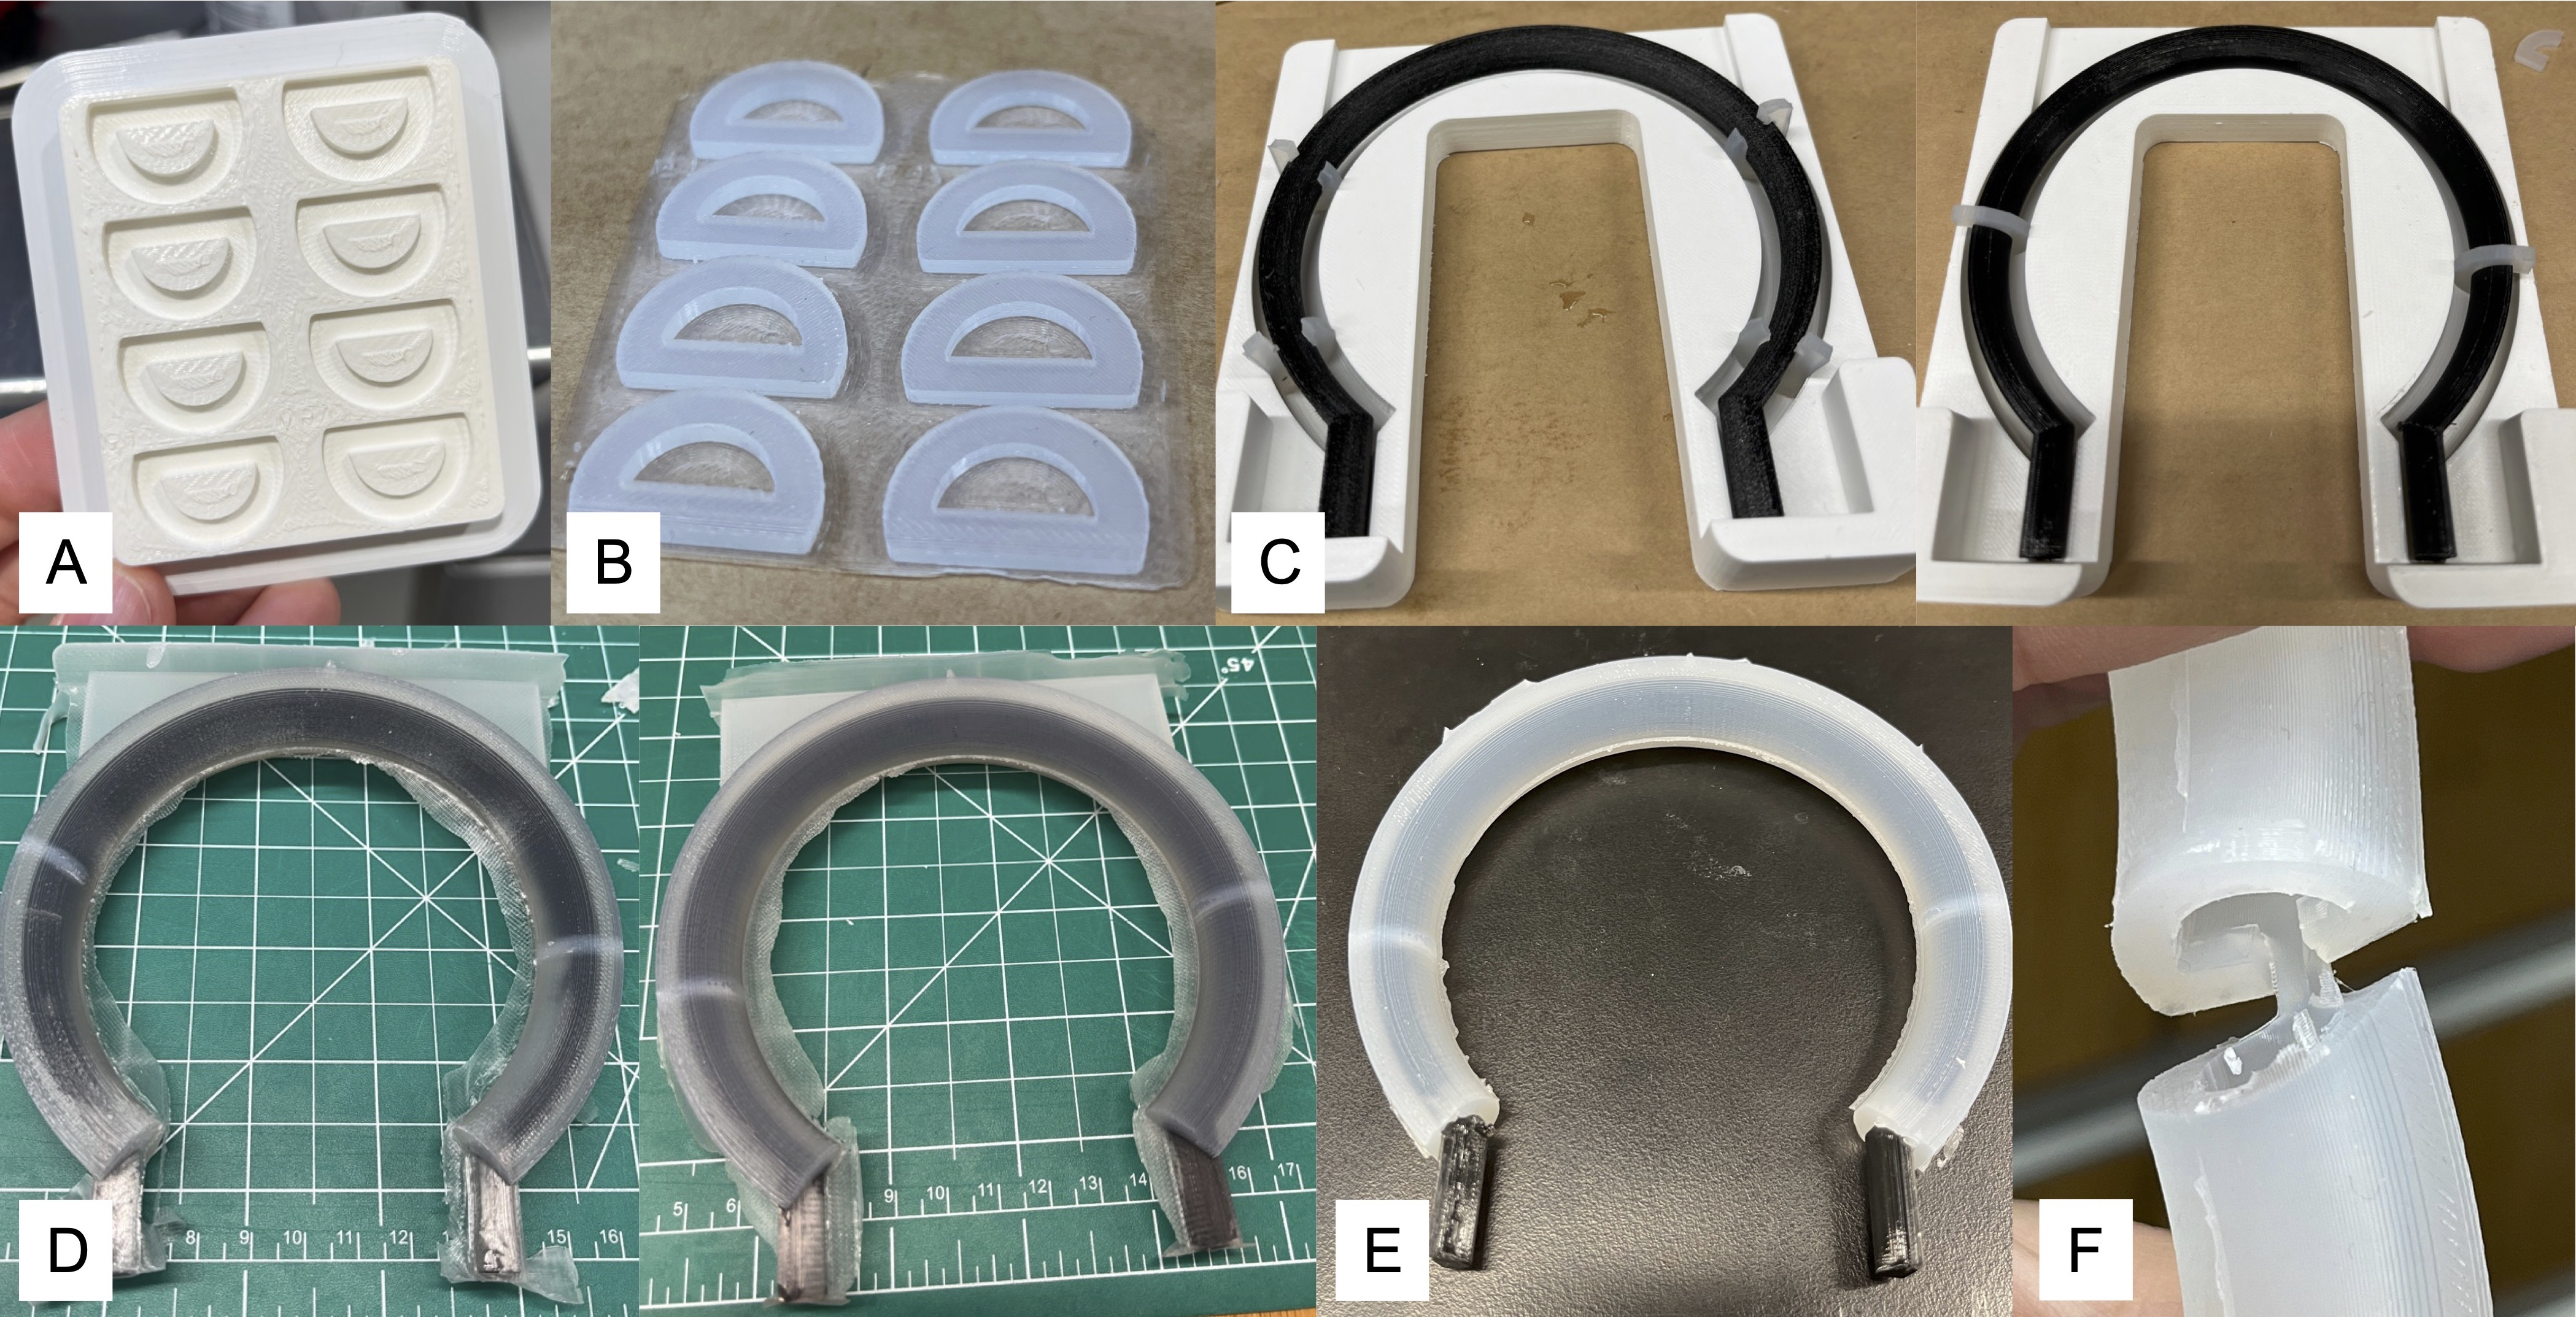
\includegraphics[width=5.5 in]{images4/ds20spacer.jpg}
    \caption{Images of failed attempts at using a spacer made from DS20 silicone to center the TPU insert. A. 3D printed mold for the spacers. B. Casted spacers. C. Arbitrary placement of spacers. D. Casted actuators right after removing from the mold. E. After removing excess silicone. F. Failed attempt at creating a seal.}
    \label{fig:ds20spacer}
\end{figure}

Overall, iterating with a flexible insert reaffirmed the need to cast the actuator's body in as few pours of silicone as possible to ensure the actuator would be airtight. Additionally, just because the insert works for the soft DS20 silicone does not necessarily guarantee that the insert will work for stiffer silicones. 

\clearpage
\subsection{Wax Inserts}

We fabricated wax inserts to create an insert that is more rigid than TPU but not as wasteful as PVA. We found three waxes compatible with curing silicone: beeswax, paraffin wax, and microcrystalline wax. We decided to cast the wax in a silicone mold for easy removal. To cast the silicone used as a mold, we 3D-printed a mold and insert out of PLA. Fig. \ref{fig:waxinserts} contains images from experimenting with wax inserts. 

\begin{figure}[ht]
    \centering
    \includegraphics[width=5.5 in]{images4/waxinserts.jpg}
    \caption{Experimentation with wax inserts. A. 3D printed mold and insert for casting silicone mold for wax. B. Casting silicone mold. C. Paraffin wax casting. D. Paraffin insert removed from mold. E. Beeswax and microcrystalline wax casting. F. Beeswax and microcrystalline wax inserts.}
    \label{fig:waxinserts}
\end{figure}

All three waxes could be partially cast and removed from the silicone mold. However, we found that creating the wax insert to have the perfect cross-section shape to ensure a future uniform cross-section for the actuator was difficult, and the waxes were not rigid enough to hold their shape inside the DS20 mold during casting. We considered combining waxes in different ratios to enhance the stiffness and ease of casting. However, even if the wax inserts could create the perfect cross-section when casting silicone, they must be melted and recast to fabricate each actuator. With mass production in mind, we decided not to pursue wax inserts. 

\subsection{Two-Part PLA Inserts}

Reexamining the requirements for the insert design, we want an insert we could use for multiple actuators, and that creates a constant cross-section along the actuator. For the TPU insert, the ends with a different geometry than the cross-section of the actuator could not slide through stiffer silicones. If we split the insert along the section with the semi-circular cross-section, we could remove each part of the insert separately, and the silicone would not have to stretch during this process. 

To align the parts of the insert with each other, we added a connection point in the middle of the insert. Because the casted silicone picks up the filament lines, and 3D-printing the inserts with the large overhang without support material would cause inconsistencies in the cross-section, we attempted printing inserts in several orientations. Fig. \ref{fig:splitinsert} contains photographs of the possible orientations for 3D printing the split insert and actuators fabricated with this method. After 3D printing, we would also file and sand the inserts to ensure a smooth surface for the silicone to cast around. Fig. \ref{fig:splitinsert}A and B's 3D-printing orientation was difficult to smooth because the orientation of the layers meant more lines of filament on the sides of the insert, which made the silicone uneven on the inner wall. Fig. \ref{fig:splitinsert}C's orientation, the same method used for printing the PVA and TPU inserts, was the best because the lines of filament were aligned with the length of the actuator, creating a smoother inner surface. We use Teflon tape, which has a small width and smooth surface, to seal the interface between the two halves of the insert. \\

\begin{figure}[ht!]
    \centering
    \includegraphics[width=6.5 in]{images4/splitinsert.jpg}
    \caption{Photographs of the 2 part insert method. A-C. Three orientations for 3D printing the insert. D-G. DS20, DS30, SS40, and SS50, respectively, cast using inserts printed in the orientation shown in C.}
    \label{fig:splitinsert}
\end{figure}

\clearpage
\section{Adding Strain Limiting Materials}

Now that we could consistently create circular actuators with a uniform cross-section in a single pour, the next problem was attaching the fiberglass fabric to the flat side of the silicone, a requirement for achieving the desired bending behavior with actuation. We used a large fiberglass fabric sheet (4 oz S-glass, US Composites) and cut it into strips slightly wider than the actuator to cover the entire flat face in fibers. We used Sil-Poxy (Smooth-On) to adhere the fabric to the silicone. We left the rigid PLA inserts inside the actuator while attaching the fiberglass fabric to ensure we added no stress to the silicone. Additionally, the fibers were attached parallel to the actuator to ensure the strain would be limited axially. If the fibers in the fabric are not aligned with the axial deformation the fiberglass is designed to restrict, the actuator will bend and twist in different directions with pressurization. 

Unfortunately, the Sil-Poxy adhesive was not strong enough on its own to keep the fiberglass attached, so we had to develop a way of covering the fabric in silicone to ensure the fabric would not become loose against the exterior of the actuator. In the standard fiber-reinforced actuator, a thin silicone wall is cast around the fiberglass, encasing the entire actuator. 

We attempted to design wider arch-shaped molds to cast another layer of silicone around the fiberglass, but this method was unsuccessful. Ensuring the second silicone cast had no air bubbles and completely covered the actuator was challenging due to the desired wall thickness. Additionally, making the walls of the actuator thicker would require more air pressure to achieve the bending behavior. For the softer silicones, casting another layer would be possible, but for the thicker silicones, such as SS40 and SS50, pouring another layer would be next to impossible. We considered casting an outer layer of a different material around the actuator, such as a thin Ecoflex silicone. However, having the semi-circular cross-section made from two different materials adds unnecessary complexity. 

To keep the total fabrication time as fast as possible, we used DragonSkin 10 (DS10) Fast cure silicone to paint a thin layer over the fiberglass fabric. Fig. \ref{fig:fiberglass} contains photographs of actuators before adding the fiberglass and after coating the fabric with a thin layer of DS10 silicone. The cure time for the DS10 silicone is under 1 hour, and only a small amount is needed to encase the fiberglass. We placed the actuator with the coat of DS10 on the table to dry, which allowed gravity to make the wall of silicone thin, but left a small amount of DS10 on the side of the actuator resting on the table (Fig. \ref{fig:fiberglass}D). This method was simple to execute repeatably, allowing for a consistent connection between the fiberglass fabric and the silicone actuator. 

\begin{figure}[ht!]
    \centering
    \includegraphics[width=5.5 in]{images4/fiberglass.jpg}
    \caption{Process of adding strain limiting fiberglass: A. Cut away silicone from flat side. B. After adding fiberglass to an SS40 actuator. C. After adding fiberglass to DS20. D. DS20 actuator right after the DS10 cured. E. After removing excess DS10.}
    \label{fig:fiberglass}
\end{figure}

\clearpage
\section{Sealing the Ends}

The easiest method to seal the ends is to place each end of the actuator in a cup full of silicone. While this method is the simplest, the amount of silicone pulled up the hollow actuator due to capillary effects is difficult to control. The larger the amount of silicone that forms the end cap, the more the final actuator's length decreases, which reduces the initial bending angle of the circular actuator. Additionally, there is an extra step to cut away the excess silicone cured around the end, leaving an end that is not necessarily uniform with the rest of the actuator. 

To ensure only the necessary amount of material cures inside the end of the actuator to create the end cap and maintain the actuator's clean cross-section, we designed and 3D printed a mold that matches the curvature of the circular actuator. Using these molds allowed us to cap the ends of all of our actuators with the same thickness on each end, further ensuring uniformity between the actuators. Fig. \ref{fig:endcaps} contains photographs of sealing the ends of the actuators and a drawing of the custom end cap mold used for the circular actuator. 

\begin{figure}[ht!]
    \centering
    \includegraphics[width=6 in]{images4/endcaps.jpg}
    \caption{Methods for sealing the ends of the actuator. A. Using a cup. B. Drawing of the custom mold. C. Sealing one end using the custom mold.}
    \label{fig:endcaps}
\end{figure}

\clearpage
\section{Connection to Pressurization Equipment}

We used standard tubing and push-to-connect fittings with 10-32 male threads to connect the actuator to the pressurization equipment. Fig. \ref{fig:barb} contains photos of the vented screw method and our custom barbs for connecting the actuator to the pressurization equipment. The vented screw method \cite{polygerinos_modeling_2015} involves using two pieces of laser cut acrylic, a vented screw, and a 10-32 nut to tighten the acrylic pieces around the end cap of silicone (Fig. \ref{fig:barb}C). Installation requires puncturing the vented screw through the inside of the actuator (Fig. \ref{fig:barb}A-B). A 10-32 female standoff connects the vented screw to the push-to-connect fitting (Fig. \ref{fig:barb}D). 

This method was successful for softer silicones, such as DS20. However, for stiffer silicones, puncturing with the vented screw often created a large hole in the end cap (Fig. \ref{fig:barb}B), which we attempted to seal with silicone glue with varying success. Additionally, puncturing from the inside, which requires feeding the vented screw through the entire length of the actuator, would prove difficult if we ever wanted to make the actuator longer and possibly spiral-shaped. 

To simplify the connection to the push-to-connect fitting, we designed and machined several barbs (Fig. \ref{fig:barb}E) from brass with 10-32 female threads that directly connected to the push-to-connect fittings (Fig. \ref{fig:barb}F). There are multiple benefits to using the barb over the vented screw. Firstly, the barb provided a way to clamp the actuator during testing. Also, puncturing the actuator from the outside allowed us to simplify the fabrication process further because we could cast the silicone on both end caps at the same time. Additionally, we have more control over the location of the puncture hole because we can see the insertion point. 

After puncturing the barb into the actuator, we used Sil-Poxy adhesive both underneath and around the brass barb to ensure an airtight connection. Also, we used a small amount of Kevlar thread to tie the end cap around the spikes of the barb. Adding the thread proved to be the most effective way of ensuring an airtight connection. 

\begin{figure}[ht!]
    \centering
    \includegraphics[width=5 in]{images4/barb.jpg}
    \caption{Methods for connecting the actuator to pressurization equipment. A. Vented screw and inner piece of acrylic. B. Large puncture hole for the stiffer SS45 silicone. C. Airtight DS20 actuator. D. 10-32 female standoff and push-to-connect fitting. E. Barbs machined for the circular actuator. F. Direct connection to push-to-connect fitting. G. Airtight SS50 and DS30 actuators. }
    \label{fig:barb}
\end{figure}
\chapter{Pressure Rig}

\section*{Preface}

Thank you to Michael Giglia and Isaiah Rivera, the design and construction of the pressure rig would not have been possible without their contributions. 

\section{Overview}

We designed the pressure rig to actuate and control the pressure inside the soft robots presented in this work. The rig contains an air tank reservoir that stores pressurized air generated from a compressor. The reservoir supplies air to a pressure regulator that controls the input pressure of the soft robot. A microcontroller ($\mu$C) controls both the regulator and compressor. The computer running the test script either takes a photograph or a force reading at each pressure increment. Fig \ref{fig:blockdiagram} contains a block diagram detailing the pressure rig and the sensors used to characterize the behavior of the circular actuators. This chapter details the mechanical components, the electrical components, firmware on the microcontroller through two iterations of the rig, and the testing scripts used to characterize bending angle and blocked force. 

\begin{figure}[ht]
    \centering
    \includegraphics[width=5.5 in]{images6/blockdiagram.jpg}
    \caption{Block diagram of the pressure rig showing the path of compressed air, the relevant control signals, and the sensors used for characterization of the circular actuator.}
    \label{fig:blockdiagram}
\end{figure}

\section{Air Supply Components}

The air tank reservoir (LYH-1004, Longyihong) has a half-gallon capacity rated for 200 PSI, well over any pressures used in this work. On each side of the tank, there is a 1/4" NPT port. One side of the tank is connected to the compressor (202, GSPSCN). On the other side of the tank, we use a 2-way, 5-port manifold block (ML-G, Baomain) to connect one of the pressure sensors, the supply of the pressure regulator, the 45 PSI pressure-relief valve (9889K19, McMaster) and the 0-50 PSI gauge (0-50PSI HF, Meanlin Measure). 

The pressure regulator (ITV1031-21N2N4, SMC) requires a 12V power supply and an input signal of 0-5V for the pressure on the output. The display shows the pressure in PSI. Both the pressure regulator and the compressor are powered by a rechargeable 12V lead-acid battery (ML5-12, Mighty Max Battery). We charged the battery often to maintain its health. We placed an E-Stop button (YW1B-V4E02R-BOX, Twtade) between the battery and the regulator. Fig. \ref{fig:airsupply} contains a photograph of the pressure rig with labeled air supply components. 

To ensure no air leaks occurred, we used Teflon Tape to secure the connections between the components. We used white 1/4" diameter tubing and 1/4" NPT to 1/4" OD tubing push-to-connect fittings (PC-1/4-N2, Tailonz Pneumatic) to connect the manifold block to the pressure regulator and pressure sensor. We used laser-cut acrylic pieces and standoffs to lift all of the components off the metal testing table. 

\begin{figure}[ht]
    \centering
    \includegraphics[width=3.5 in]{images6/airsupply.jpg}
    \caption{Photograph of the pressure rig with air supply components labeled.}
    \label{fig:airsupply}
\end{figure}

\section{Pressure Sensor}

The differential pressure sensor (MPX2200DP, Freescale Semiconductor) measures the pressure within the air tank to ensure the regulator has sufficient air supply. We used readings from this sensor to turn the compressor on or off. To connect the pressure sensor to the microcontroller, we used an instrumental amplifier (INA125P, Texas Instruments) and a 13-bit analog-to-digital converter with an SPI serial interface (MCP3301, Microchip). Both microcontrollers had SPI communication libraries written to interface with the pressure sensor. 

\section{Compressor Control}

We designed the compressor to be controlled by the microcontroller using a digital pin connected to an NMOS (IRF540N), which connects to a relay to connect the compressor to the battery. Using the pressure sensor reading of the air tank, we wrote a state machine that controls the pressure so that the tank remains full while testing the actuators. Fig \ref{fig:compressorsm} contains a diagram of the state machine that runs on either microcontroller to control the compressor. 

\begin{figure}[ht]
    \centering
    \includegraphics[width=6 in]{images6/compressorsm.jpg}
    \caption{State machine diagram for compressor control to fill the air tank.}
    \label{fig:compressorsm}
\end{figure}

The state machine has 3 states, compressor OFF (state 0), compressor ON (state 1), and ESTOP (state 2). While in state 0, we check if the current pressure reading in the tank is less than the desired pressure minus some tolerance. If the pressure has dropped below this amount, switch to state 1, and the compressor turns on. In state 1, we check if the dP/dt (the change in pressure over time) is satisfactory, such that we know there is no air leak. We use timing functions in firmware to check the current pressure compared to the pressure reading each time increment before. If dP/dt is less than expected, we can assume there is a leak and the compressor is not filling up the tank; in this case, switch to state 2, the emergency stop state. If dP/dt increases as expected, check if the current pressure is above the desired pressure plus some tolerance. If so, switch to state 0 and turn the compressor off. 

The allowable tolerance of the tank pressure provides a small buffer, ensuring the compressor does not turn on and off frequently, prolonging its life. We used 36~$\pm$~4~psi (250~$\pm$~35~kPa) as the desired tank pressure for experimentation. 

\section{Input to Pressure Regulator}

The regulator's output pressure range is programmable. To stay within the release valve's bounds, we set the output pressure to be between 0 and 40 PSI. 
The analog input signal (0-5V) has a linear relationship between voltage and output pressure from the regulator. We used a digital potentiometer with an SPI serial interface (MCP4251-103E/P, Microchip) connected to the Arduino (ELEGOO UNO R3) in the first iteration. In the second iteration, we used a 12-bit digital-to-analog converter, also with an SPI interface, connected to the Pico microcontroller (Raspberry Pi). 

\subsection{Sending Pressure Commands to Arduino}

Using an Arduino microcontroller, we controlled the digital potentiometer, creating the analog voltage signal that controls the pressure output from the pressure regulator. The microcontroller and the digital potentiometer communicated over SPI. However, we wanted to be able to set the desired pressure using the computer running the test script. The computer connects to the camera and force sensors. We wrote the testing script in Python to step between pressure increments so that we could either take a photograph of the bending angle or record the blocked force using the load cell. In between taking a photograph or force reading, the computer sends pressure commands to the microcontroller to change the pressure inside the actuator. 

We used a custom g-code-like serial protocol Michael Giglia had previously implemented and modified it to send the desired pressure commands. At the time, we were using the 8-bit signal to the digital potentiometer, so the message sent from the Python script to the $\mu$C was a number between 0-255. After determining the appropriate commands and the pressure output at those commands, we wrote a testing script that would iterate through each pressure command and take a photograph or force reading when the person taking the data indicated that the actuator had reached a steady state at that pressure. 

\subsection{Problems with the Digital Potentiometer}

The digital potentiometer used to create the analog voltage as the input signal to the pressure regulator was problematic due to the non-linear results of controlling it with the Arduino. 

To set the pressure in the actuator, we sent an 8-bit command (0-255) from the computer running the test script to the Arduino. We attempted to characterize the non-linear relationship between the range set on the pressure regulator, the command sent to the digital potentiometer, and the output pressure. Fig. \ref{fig:bitpressuremap} contains the pressure readings based on the command sent to the digital potentiometer at 4 different ranges of the pressure regulator. Because the resolution at higher pressures was significantly lower, we increased the range on the pressure regulator to gain more resolution at higher pressures. The silicone actuators were highly sensitive to pressure changes, and we found worse hysteresis in the bending angle when the pressure increments were highly uneven. 

\begin{figure}[ht]
    \centering
    \includegraphics[width=6 in]{images6/bitpressuremap.jpg}
    \caption{Relationship between the range set on the pressure regulator, the command sent to the digital potentiometer and the output pressure in the actuator for four pressure ranges.}
    \label{fig:bitpressuremap}
\end{figure}

\clearpage
\subsection{Digital to Analog Converter}

It was critical to have linear control over the output pressure of the pressure regulator to increase or decrease the pressure in the actuator by an even amount. To achieve linear output pressure, we needed a way to create an analog 0-5V signal with linear input commands with the desired output pressure. We achieved linear control between the command and the output pressure by implementing a 13-bit digital-to-analog converter (MCP4921-E/P, Microchip) using an SPI interface with a Pico microcontroller. This upgrade allowed us to measure the circular actuator's bending and blocked force behavior with even pressure increments, critical to minimizing hysteresis during characterization. 

\subsection{Problems with Switching to the Pico}

Switching microcontrollers required a complete overhaul of the testing software and firmware. Isaiah Rivera rewrote and rebuilt the pressure rig to have the upgraded microcontroller driving it. Still, because we switched to the digital-to-analog converter to control the regulator's output, we had to write the SPI communications for the new device, and we wanted to move to the Pico. Hence, we decided to upgrade the entire rig. 

Due to time constraints and an oversight of how much development would be required to change microcontrollers, we simplified the pressure rig. We used one Pico $\mu$C to control the compressor. The pressure sensor interface and compressor control state machine always ran while the rig was on. We used a second Pico $\mu$C to interface with the pressure regulator. Instead of waiting for the serial protocol implementation, we decided to use a potentiometer input, using the Pico's analog-to-digital converter to control the pressure output of the regulator. While this solution certainly requires several layers (a 3.3V analog signal is read by the Pico, converted to a digital value, and sent over SPI to a digital-to-analog converter, which creates a 0-5V analog signal to set the regulator's pressure), it did work. It allowed us to take both bending angle data and blocked force data at even pressure increments, which was the most important part of characterization. 

We discretized the potentiometer readings into even increments to ensure the same pressure commands were sent for each actuator's test. The new setup using the digital-to-analog converter provided immense resolution on the pressure regulator's output, but we wanted to use 1 psi increments. Since now the relationship between the signal sent to the DAC and the pressure output on the regulator was linear, it was simple to discretize the values so that we had even increments of 1.0~$\pm$~0.1 psi. 

Since we had lost the serial protocol between the $\mu$C and the computer, the testing script had to be modified to print the desired pressure to the terminal output. The person running the test would turn the potentiometer until the regulator received the desired pressure command. A photo or force reading could be taken once the actuator had reached a steady state. Despite taking slightly longer to run each test, the hysteresis caused by uneven pressure increments was greatly reduced, making the switch to the Pico worth it. 

\clearpage
\section{Camera for Bending Angle}

To experimentally measure the bending angle of the circular actuators, we used a camera to take photos of the actuator at each pressure. We entertained using a flexible resistor (SEN-08606, SparkFun), but this would not provide insight into variations in curvature or non-axial expansion along the length of the actuator. A photograph, although requiring post-processing, provides infinite insight into the actuator's bending behavior. 

We used a web camera (C920 Hd Pro, Logitech) to take photographs of the actuator at each pressure. Our testing script used OpenCV \cite{opencv_library} to interface with the web camera and save the photographs in the appropriately named directory for later post-processing. 

For each test, the person running the test would input the \emph{name} of the actuator and the number of the test. For example, DS20K3\textunderscore4 meant the actuator was made of DragonSkin 20 silicone, it was fabricated with the K method (the insert split in the center of the actuator), it was the third actuator made with this material and fabrication method, and this is the fourth time running the bending angle experiment. 

Using the terminal output and keyboard of the computer, the person running the test would see the pressure about to be sent to the actuator and then press the space bar to confirm the pressure should be changed. Once the actuator had reached a steady state at that pressure, pressing the ``m" key would take a photograph, name it with the name of the actuator and the current pressure, and save it to a directory with the name of the test. The script would continue through the list of pressures we wanted to test the actuator at until the peak pressure was reached. After documenting the bending angle at the maximum pressure, the pressure would reverse to capture hysteresis in the bending behavior. Each test took 5-10 minutes to take 30-35 photographs, depending on the achievable peak pressure in the actuator. Chapter \ref{chapter:bendingangle} fully details capturing the bending angle of the circular actuator. 

\section{Load Cell for Blocked Force}

To determine the size of the load cell required to characterize the blocked force of the circular actuators, we used the scale used to weigh the silicone during casting. We determined that a 2~kg load cell would not saturate while measuring the blocked force when we blocked the actuator from unbending. 

We used a 2~kg load cell (a14071900ux0069, Uxcell) connected to an amplifier (CJMCU-711 HX711, Cylewet). This amplifier has digital communications using the DATA and CLK pins. Instead of using the microcontroller to take the force readings, we used the computer and a USB to GPIO converter (CJMCU FT232H, Koobook). We took the average of 100 load cell readings for each force reading. Using the computer was advantageous because we could switch microcontrollers without changing how we recorded force data. Chapter \ref{chapter:blockedforce} fully details the blocked force characterization for the circular actuator. 




\chapter{Analytical Model For Bending Angle}
\label{chapter:model}

To characterize the actuator's bending behavior as a function of input pressure and material properties, we developed an analytical model for curling and uncurling based on those found in \cite{polygerinos_modeling_2015, connolly_automatic_2017, hu_precurved_2022}. We calculate the input pressure $P$ required to reach a given bending angle $\psi$ using the geometry of the actuator, the length of the inextensible layer $l_0$, and the non-linear hyperelastic material properties of each silicone, including non-axial deformation. To account for circumferential deformation, we transform the cross-section at each pressure based on material stretches. As the pressure increases, the actuator uncurls (decreasing $\psi$) from its initial bending angle $\psi_0$ to an angle $\psi=0$, where the actuator is straight. Further increasing pressure causes $\psi$ to become negative, corresponding to curling behavior, thus generating a bi-directional range of motion. Fig. \ref{fig:modelall} contains all of the variables used in the analytical model. 

\begin{figure}[ht]
    \centering
     \includegraphics[width=6 in]{images5/modelall.jpg}
    \caption{Geometric variables defined for the analytical model. The thicker line represents the inextensible layer. A. Definition of positive and negative bending angles. B. Undeformed cross-sectional geometry of the actuator. C. Axial stretch ratios and corresponding stress in response to applied pressure. D. Deformed cross-sectional geometry to account for circumferential and radial deformation.}
    \label{fig:modelall}
\end{figure}

\clearpage
\section{Stretch Ratios}

As the actuator bends, the silicone stretches in the axial direction to maintain the length $l_0$ of the inextensible layer. The model assumes that the actuator maintains a single, constant bending radius along its length at all pressures and that the cross-section remains orthogonal to the inextensible layer. We also assume incompressibility in the hyperelastic material, such that $\lambda_{1}\lambda_{2}\lambda_{3} = 1$ where $\lambda_i$ is the stretch ratio in each direction (axial, circumferential, and radial, respectively). This assumption requires that the cross-sectional area of the silicone remains constant, even as the shape deforms. Increasing pressure causes the semi-circular region to expand outwards into a circular shape, resulting in thinning of the actuator's walls to maintain a constant cross-sectional area (Fig. \ref{fig:modelall}D). We assume no geometric changes in the base layer because of the proximity to the inextensible layer.

For the undeformed cross section, as shown in Fig.~\ref{fig:modelall}B, $\beta$ is the coordinate in the base layer away from the inextensible layer, and $\tau$ is the distance from the inner wall in the $\varphi$ direction. The base region has thickness $b$~=~0.38~cm, and the undeformed semi-circular cross-section wall has radius $a_0$~=~0.64~cm and thickness $t_0$~=~0.38~cm. In the deformed cross-section (Fig.~\ref{fig:modelall}D), we assume that the silicone forms a circular arc with offset from the base $q$, inner radius $a$, wall thickness $t$ and angle range $-\varphi_m$ to $\varphi_m$. $\tau'$ and $\varphi'$ are scaled coordinates with reference to the undeformed shape such that $\tau'=\tau\frac{t}{t_0}$ and $\varphi'=\varphi\frac{2\varphi_m}{\pi}$.

For a given bending angle $\psi$, we calculate the axial stretch ratio $\lambda_1$ as $\lambda_{\beta}$ for material in the base and $\lambda_{\varphi,\tau}$ in the semi-circular region (Fig.~\ref{fig:modelall}C). When $\psi$ is negative, the axial stretch ratio remains positive as all lengths must exceed $l_0$. We also calculate the circumferential stretch ratio based on the deformed cross-section. These equations hold for the entire range of $\psi$ and deformation of the cross-section. 

\begin{equation}
    \lambda_1=\lambda_{\beta} = \frac{l_{0} - \beta \psi}{l_{0}-\beta\psi_0} 
    \label{eq:stretchbeta}
\end{equation}

\begin{equation}
    \lambda_1=\lambda_{\varphi,\tau} = \frac{l_{0} - (b+q+(a+\tau')\cos\varphi')\psi}{l_{0} - (b+(a_0+\tau)\cos\varphi)\psi_{0}}
    \label{eq:stretchphitau}
\end{equation}

\begin{equation}
    \lambda_2=\lambda_c = \frac{2(a+\tau')\varphi_m}{(a_0+\tau)\pi} 
    \label{eq:stretchc}
\end{equation}

For the undeformed shape, the circumferential stretch ratio $\lambda_2$ is 1. The stretch ratio in the radial direction $\lambda_3=\lambda_r$ can be calculated as $\lambda_3=1/(\lambda_1 \lambda_2)$ from the incompressibility assumption. To find the wall thickness $t$ of the circular arc region of the deformed cross-section, we integrate the radial stretch of the undeformed shape over the thickness:

\begin{equation}
    t = \int_0^{t_0} \frac{1}{\lambda_{\varphi,\tau} \times 1} d\tau 
    \label{eq:thicknessfromlambdar}
\end{equation}

To account for the inaccuracy of the material models and the compressibility of the DragonSkin materials, we scale the calculated thickness by $k_t(1-|\psi-\psi_0|/\psi_0)$ where $k_t = 0.3$ is a constant determined by best fit to the experimental expansion results. This scaling accounts for the non-zero radial stress, especially at negative bending angles. No scaling is necessary for the stiffer SmoothSil materials. 

To transform the cross-section from the original semi-circle to the circular arc, we use the scaled thickness $t$ and the cross-sectional area $A_0$ to calculate the deformed inner radius $a$, angle range $2\varphi_m$, and vertical offset $q$:

\begin{equation}
    \frac{A_0}{2\sin{\varphi_m}t}-\frac{t}{2}=\frac{a_0}{\sin{\varphi_m}}
    \label{eq:phi_m}
\end{equation}

\begin{equation}
    a=\frac{A_0}{2t\varphi_m}-\frac{t}{2}
    \label{eq:a_aug}
\end{equation}

\begin{equation}
    q=-a\cos{\varphi_m}
    \label{eq:q_aug}
\end{equation}

The axial and circumferential stretch ratios are then recalculated using the deformed cross section and Equations \ref{eq:stretchbeta}--\ref{eq:stretchc} before calculating stress with the material models.

\section{Converting Strain to Stress}

To describe the stress-strain relationship for each of the soft materials, multiple material models are available; they can vary significantly in accuracy depending on the amount of strain \cite{paterno_hybrid_2018}. We choose the Ogden hyperelastic material model because it is more accurate at higher stretches and for softer materials \cite{marechal_toward_2021}. The strain energy density function $W$ for the Ogden model is given by Eq. \ref{eq:strain-ogden}, where $\mu_{p}$ and $\alpha_{p}$ are experimentally determined material coefficients. We can use a given Neo-Hookean material model coefficient ($\mu$) in the Ogden model by setting $N=1$ and $\alpha_1=2$. 

\begin{equation}
    W=\sum_{p=1}^N \frac{\mu_p}{\alpha_p}(\lambda_1^{\alpha_p}+\lambda_2^{\alpha_p}+\lambda_3^{\alpha_p}-3)
    \label{eq:strain-ogden}
\end{equation}
\\
The Cauchy stresses in all three directions are given by $\sigma_j=-p+\lambda_j\frac{\partial W}{\partial\lambda_j}$, where $p$ is a Lagrange multiplier. The stresses in the radial direction are significantly smaller than those in the other directions, so we assume $\sigma_3=0$. We calculate the axial and circumferential stresses using Equations \ref{eq:s_1} - \ref{eq:multiplier-p} and the material properties found in Table \ref{table}. 

\begin{equation}
    \sigma_1 =-p+\mu_1\lambda_1^{\alpha_1}+\mu_2\lambda_1^{\alpha_2}+\mu_3\lambda_1^{\alpha_3}
    \label{eq:s_1}
\end{equation}

\begin{equation}
    \sigma_2 =-p+\mu_1\lambda_2^{\alpha_1}+\mu_2\lambda_2^{\alpha_2}+\mu_3\lambda_2^{\alpha_3}
    \label{eq:s_2}
\end{equation}

\begin{equation}
    p=\mu_1(\lambda_1\lambda_2)^{-\alpha_1}+\mu_2(\lambda_1\lambda_2)^{-\alpha_2}+\mu_3(\lambda_1\lambda_2)^{-\alpha_3}
    \label{eq:multiplier-p}
\end{equation}

\begin{table}[h!]
\caption{Material Properties Used in Analytical Model}
\label{table}
\centering
\begin{tabular}{l r r l}
\hline
{} & \bfseries Variable & \bfseries Value & \bfseries Unit \\
\hline\hline
DS20 \cite{marechal_toward_2021} & $\mu_1$, $\mu_2$, $\mu_3$ & -0.9534, -1.4515, 2.4085 & MPa\\
{} & $\alpha_1$, $\alpha_2$, $\alpha_3$ & 3.478, 3.181, 3.339 & {}\\
\hline
DS30 \cite{marechal_toward_2021} & $\mu_1$, $\mu_2$, $\mu_3$ & 0.03816, 0.02524, 0.04456 & MPa\\
{} & $\alpha_p$ & 3.417 & {}\\
\hline
SS40 \cite{pagoli_review_2022} & $\mu_1$ & 0.24 & MPa\\
{} & $\alpha_1$ & 2 & {}\\
\hline
SS50 \cite{xavier_finite_2021} & $\mu_1$ & 0.68 & MPa\\
{} & $\alpha_1$ & 2 & {}\\
\end{tabular}
\label{table}
\end{table}

\clearpage
\section{Pressure from Bending Moments}

The bending moments $M_P$ and $M_\sigma$ about the \(O\) axis (Fig.~\ref{fig:modelall}C) result from pressure on the end of the actuator and axial stress, respectively. These moments must be equivalent for the actuator to achieve static equilibrium. We calculate the bending moment $M_\sigma$ as the integral of the force from axial stress in both the base ($\sigma_{\beta}$) and the circular arc ($\sigma_{\varphi, \tau}$) regions times the orthogonal distance from \(O\) for the entire length of the actuator. 

\begin{equation}
    M_{\sigma} = 2l_{0} \int_{0}^{b} \sigma_{\beta} (a_0+t_0) \beta  d\beta
    + l_{0}\int_{0}^{t_0}\hspace{-2px}\int_{-\frac{\pi}{2}}^{\frac{\pi}{2}}\hspace{-2px}\sigma_{\varphi,\tau}((a+\tau')\cos{\varphi'}+b+q)(a+\tau') d\varphi d\tau
    \label{eq:moment-axial}
\end{equation}

The bending moment $M_P$ resulting from a given input pressure \(P\) acting on the end of the actuator is a function of the deformed cross-sectional geometry: 

\begin{align}
    M_P & = P \int_{-\frac{\pi}{2}}^{\frac{\pi}{2}}\int_0^{a} a(b+q+a\cos{\varphi})d\varphi da \\ \nonumber \\
    & = \frac{4 a^{3} + 3 \pi a^{2} (b+q)}{6} P 
    \label{eq:moment-p}
\end{align}

We equate (\ref{eq:moment-axial}) and (\ref{eq:moment-p}) and solve for the required input pressure $P$ to induce the axial stresses for a given bending angle $\psi$. To account for the underestimation of $P$ due to uncertainty in the material models and non-uniformity in the actuator, we scale the calculated pressure by a constant $k_P$, determined by a best fit for each material. $k_P$ is 3.8 for DS20, 1.8 for DS30, and 2.2 for SS40 and SS50. 

\clearpage
For each material's initial bending angle, $\psi_0$, we chose the average value from all actuators fabricated with that material (between 214-228$^\circ$). Fig. \ref{fig:modelresults} contains the bending angle at each pressure calculated with the analytical model for DS20, DS30, SS40, and SS50 materials. 

\begin{figure}[!ht]
    \centering
    \includegraphics[width=6.5 in]{images5/modelresults.pdf}
    \caption{Analytical model for bending angle for circular actuators of four materials.}
    \label{fig:modelresults}
\end{figure}
\chapter{Measuring Bending Angle}
\label{chapter:bendingangle}

\section*{Overview}
This chapter contains how we measured the bending angle of the circular actuators at different pressures, the equipment used, the various orientations we used to photograph the actuator, testing protocols, how we processed the images, and how we calculated the bending angle.

\section{Photographing Bending Angle}

To experimentally measure the bending angle of the circular actuators, we used a camera to take photos of the actuator at each pressure. We entertained using a flexible resistor (SEN-08606, SparkFun), but this would not provide insight into variations in curvature or non-axial expansion along the length of the actuator. A photograph, although requiring post-processing, would allow us to characterize the bending behavior. We used a web camera (C920 Hd Pro, Logitech) to take photographs of the actuator at each pressure.

\section{Iterations on Orientation}

As with everything related to this project of designing and characterizing a new type of soft robotic actuator, discovering how to measure the bending angle at different pressures repeatably took several iterations. We needed to develop a way to hold the actuator in front of the camera so we could measure the bending angle and compare it to the model. Since the fiberglass fabric embedded into the actuator determines the bending angle, the camera must be placed perpendicular to the fabric. We also wanted to capture the actuator's circumferential expansion in the photographs. 

Appendix \ref{appendix:ao} contains the complete process for how we determined the best orientation to photograph bending angle. Samples of the various orientations are contained in Fig \ref{fig:orientationsall} which includes testing vertically where the actuator can make contact with the table (Fig \ref{fig:orientationsall}A), horizontally where friction impacts the behavior (Fig \ref{fig:orientationsall}B), vertically with gravity (Fig \ref{fig:orientationsall}C), vertically but lifted off the table (Fig \ref{fig:orientationsall}D), and finally vertically against gravity (Fig \ref{fig:orientationsall}E). Each of these orientations suffered from external influences creating non-constant curvature in the circular actuator. 

\begin{figure}[!ht]
    \centering
    \includegraphics[width=6.5 in]{images7/orientationsall.pdf}
    \caption{Various orientations initially used to photograph bending angle. Contains photographs of DS20 actuators at 2.0, 6.0, 10.0, and 12.1 psi}
    \label{fig:orientationsall}
\end{figure}

\clearpage
\subsection{Chosen Orientation}

In order to remove the influence of gravity and friction on the bending angle as we chose to photograph the actuator horizontally. If the fiberglass fabric was placed perpendicular to the table, using a camera mounted above the table pointing down, we could capture the bending angle at any pressure. For simplicity and to not require additional hardware, we held the actuator above the table when changing the internal pressure to eliminate the effects of friction. Once the pressure regulator reached a steady state, we placed the actuator on the table before taking the photograph. Fig. \ref{fig:chosenorientation} contains photographs taken using a DS20 actuator in the chosen testing orientation. 

\begin{figure}[!ht]
    \centering
    \includegraphics[width=6 in]{images7/chosenorientation.pdf}
    \caption{DS20 actuators photographed at pressures between 0-14.5 psi.}
    \label{fig:chosenorientation}
\end{figure}

\clearpage
\section{Testing Protocols}

Using the terminal output and keyboard of the computer, the person running the test would see the pressure about to be sent to the actuator and then press the space bar to confirm the pressure should be changed. Once the actuator had reached a steady state at that pressure, pressing the ``m" key would take a photograph, name it with the name of the actuator and the current pressure, and save it to a directory with the name of the test. The script would continue through the list of pressures we wanted to test the actuator at until the peak pressure was reached. After documenting the bending angle at the maximum pressure, the pressure increments would reverse to capture hysteresis in the bending behavior. Each test took 5-10 minutes to take 30-35 photographs, depending on the achievable peak pressure in the actuator.

\section{Calculating Bending Angle}

Now that we have an effective method of photographing the circular actuators, we can use the photographs to calculate the bending angle at each pressure. Starting from the initial bending angle, $psi_0$ and rearranging the arc-length equation, $l_{0} = r_{0}\psi_{0}$, for the bending angle gives $\psi = l_0/r$, where $l_0$ is the length of the inextensible fiberglass fabric, and $r$ is the bending radius of the actuator. Measuring the curvature, $\kappa$, from a photograph of the fiberglass layer is the easiest approach to calculate the bending angle. Knowing $\kappa = 1/r$, we can calculate the bending angle from the curvature using $\psi = l_{0}\kappa$. 

\subsection{Curvature from Three Points}

Given three coordinates, $(x_1,y_1)$, $(x_2,y_2)$, $(x_3,y_3)$, in cartesian space, we can calculate the curvature of the circle formed by those three points using Eq. \ref{eq:CurvatureEq} \cite{ratliff_cartesian_2019}. 
\begin{align} 
    \kappa = \frac{2\cdot\lvert((x_2-x_1)\cdot(y_3-y_2)) - ((y_2-y_1)\cdot(x_3-x_2))\rvert}{\sqrt{[(x_2-x_1)^2+(y_2-y_1)^2] \cdot [(x_3-x_2)^2+(y_3-y_2)^2] \cdot [(x_1-x_3)^2+(y_1-y_3)^2]}} 
    \label{eq:CurvatureEq} 
\end{align}

We began by comparing the model to the experimental results using OnShape CAD software. We manually selected three points along the fiberglass layer and used the built-in functionality to measure the radius of a circle defined by three points. The checkerboard grid has 1~cm squares, which we also measured to convert the radius of the circle to meaningful units. Fig. \ref{fig:onshapecircles} contains two samples of sketches of circles created in OnShape. Note at 9.1 psi, the actuator has a positive $\psi$, and at 12.9 psi, the actuator has a negative $\psi$. Also note that as $\psi$ approaches $0^\circ$, the circle's radius approaches infinity. 

\begin{figure}[ht]
    \centering
     \includegraphics[width=6 in]{images7/onshapecircles.pdf}
    \caption{Two screenshots from OnShape with the 3 points used and the calculated bending radius, $r$ are labeled for a DS20 actuator at 9.1 and 12.9 psi.}
    \label{fig:onshapecircles}
\end{figure}

\section{Using OpenCV to Calculate Bending Angle}
\label{section:opencv}

To provide automation, we wrote a Python script using OpenCV \cite{opencv_library}. For each photograph, the script would detect the fiberglass fabric layer as a contour and use points along the contour to calculate the average curvature of the circular actuator at that pressure. 

While first developing the line-detection script, we wanted to detect both the actuator's outer and inner walls to measure the actuator's circumferential expansion. Additionally, we wanted to develop a method to measure the curvature over the length of the actuator for experimental setups where gravity or friction caused the actuator to have non-constant curvature. The first scripts utilized the black and blue checkerboard pattern to remove the distortion from the camera. Limitations of this method included not necessarily knowing which coordinates on the contour line were from the inside, outside, or end caps of the actuator. The curvature calculation requires three $x$ and $y$ coordinates from the fiberglass fabric layer. However, we needed a new method to automatically detect the correct contour and measure the bending angle. 

Measuring circumferential expansion using the photographs would provide some insight into the actuator's behavior, but ultimately, since the three strains are interconnected, measuring each strain separately provides less insight than we had hoped. After we concluded that measuring only the curvature of the fiberglass layer would provide enough information to compare to the model, we decided to use a dry-erase marker to draw a line on the silicone. We used a blue or black dry-erase marker and a white background behind the actuators to calculate the curvature with minimal post-processing. 

To convert pixels to centimeters, we photographed a ruler at several positions within the camera frame and concluded that the camera's distortion is tolerable in the center of the frame. If the actuator remained in the center of the camera frame, we could use a linear mapping between pixels and centimeters. 

Using OpenCV, we first converted the image to grayscale. Then, we applied a binary mask to isolate the line we drew on the actuator. Using the masked image, we found the contour line(s). Each contour is a list of $x$ and $y$ coordinates that compose the line. We add the coordinates to an array for curvature calculations for each detected contour. To calculate the average curvature, we first split the length of the contour into three sections. For each section, we used a random coordinate. For 100 iterations, we used the coordinates from each section to calculate the curvature. We averaged the 100 values to determine the mean curvature of the line drawn on the actuator. For each actuator, we measured the length of the fiberglass layer and converted curvature, $\kappa$, to bending angle using $\psi = l_{0}\kappa$. Fig. \ref{fig:opencvbendingangle} showcases the procedure for an SS40 actuator at 160~kPa; using coordinates along the contour line, we measured a bending angle of 102$^\circ$. 

\clearpage
\begin{figure}[ht]
    \centering
     \includegraphics[width=6 in]{images7/opencvbendingangle.jpg}
    \caption{Samples from the OpenCV script used to measure bending angle of the circular actuators. A. Original image of a SS40 actuator at 160kPa. B. Grayscale. C. Color mask. D. Random coordinates chosen from the contour line split into three sections and the calculated bending angle of 102$^\circ$.}
    \label{fig:opencvbendingangle}
\end{figure}

There are several drawbacks to this method of measuring bending angle. First, maintaining a white background was difficult, and white electric tape was often required to cover any markings created by the dry-erase markers. Also, we had to cover the brass barb and push-to-connect fitting with white electric tape. Additionally, we wanted to collect data from both sides of the actuator, so the dry-erase marker had to be cleaned off and redrawn on the other side after sufficient testing. The biggest drawback of this method of measuring bending angles is that the OpenCV script could not detect negative bending angles. Since the script reported the measured curvature, we had to manually indicate if the reported curvature corresponded to a positive or negative bending angle. 
\chapter{Bending Angle Results}
\label{chapter:angleresults}

\section{Overview}
This Chapter presents the results of bending angle experiments defined in Chapter~\ref{chapter:measurebendingangle} compared to the analytical model defined in Chapter~\ref{chapter:model}. We tested actuators made from four soft materials using the fabrication method defined in Chapter~\ref{chapter:fabrication}.

We measured the bending angle of circular actuators made from four soft materials with both increasing and decreasing pressure using $7\pm1$~kPa increments (about 1 psi). We ran six tests for each actuator and took the average value of the bending angle for all of the actuators for each material (two DS20, three DS30, three SS40, and one SS50). Fig.~\ref{fig:allmaterialvsmodel} contains bending angle results for actuators of all four materials. We present results for each material in a different color, and the shaded region represents one standard deviation of bending angle for increasing and decreasing pressure, using darker and lighter shading, respectively. Additionally, we added the bending angle predicted by the analytical model for the bending angle for each material.

\begin{figure}[ht]
    \centering
     \includegraphics[width=6.5 in]{images9/allmaterialvsmodel.jpg}
    \caption{Measured bending angle for circular actuators fabricated from four materials compared to analytical model. The shaded regions represent one standard deviation of bending angle for both increasing and decreasing pressure increments.}
    \label{fig:allmaterialvsmodel}
\end{figure}

\section{Overall Trends}

With increasing pressure, the bending angle evolved from the initially positive $\psi_0$, past $\psi=0$ when the actuator was straight, to negative bending angles, $\psi<0$, as the actuator curled back on itself. At angles near $\psi_0$, we observed little change with applied pressure as the axial and circumferential strains remained low. As the actuator approached and passed the straight $\psi=0$ point, demonstrated in the softer DS20 and DS30 actuators, rapid changes in bending angle occurred with small changes in pressure. 

Both the DS20 and DS30 actuators exhibit a total range of motion of more than double the initial bending angle within the given pressure range: 436$^\circ$ in 112~kPa and 424$^\circ$ in 175~kPa, respectively. The SS40 and SS50 actuators achieve 265$^\circ$ and 64$^\circ$ respectively in 255~kPa, the upper limit for the experimental setup.

As the bending angle decreased below $\psi=0$, the actuator's effective inner radius, $a$, grew rapidly. The circumferential expansion was no longer uniform along the length of the actuator, expanding more in the center than at the ends. This deformation created a non-constant curvature. Therefore, the larger uncertainty and asymptotic behavior at pressures above 80~kPa for DS20 and 140~kPa for DS30 could be attributed to enforcing the constant curvature assumption when calculating the predicted bending angle. 

The analytical model correctly captured the bi-directional bending behavior of the actuators, particularly the change in concavity between lower and higher strains. The RMS error between the predicted bending angle and the average experimental data, including both increasing and decreasing pressure increments, is 70$^\circ$ for DS20, 70$^\circ$ for DS30, 30$^\circ$ for SS40, and 5$^\circ$ for SS50. The larger error in the softer materials was a function of both the large hysteresis in the experimental results and the inherent uncertainty in the material models. While increasing the pressure inside the actuator, reducing the bending angle requires more pressure. After taking the actuator to the peak pressure, decreasing pressure increments meant that the actuator required less pressure for a given bending angle due to the hyperelastic material properties. Additionally, assuming incompressibility yields an underestimation of the required pressure for positive bending angles and an overestimation for negative bending angles. 

\clearpage  
\section{DS20}

DS20 actuators, the softest silicones we used in this work, had a total range of 436$^\circ$ in 112~kPa. On average, starting at an initial bending angle, $\psi_0=210^\circ$, with increasing pressure, the DS20 actuators reached $\psi=0^\circ$. They continued bending with a negative bending angle, reaching past $\psi<-\psi_0$ to a bending angle of $-226^\circ$. DS20 actuators had significant hysteresis (up to 160$^\circ$) in bending angle between increasing and decreasing pressure.

Fig.~\ref{fig:d20fewer} contains photographs of the bending angle for a DS20 circular actuator for both increasing ($P\uparrow$) and decreasing ($P\downarrow$) pressure increments. The actuator had a lower bending angle (a more negative $\psi$) for the same pressure. For this DS20 actuator, all of the photographs from this test are in Appendix~\ref{appendix:d20all}.

\begin{figure}[!ht]
    \centering
    \includegraphics[width=6.5 in]{images9/d20fewer.pdf}
    \caption{Samples of photographs used to measure bending angle of a DS20 circular actuator for both increasing and decreasing pressure increments.}
    \label{fig:d20fewer}
\end{figure}

\clearpage
Looking at 70~kPa, the pressure with the largest hysteresis (160$^\circ$), the model predicts $\psi=-70^\circ$. At this pressure, one standard deviation of DS20 actuators had a bending angle of $20\pm60^\circ$ for increasing pressure from 64~kPa and $-140\pm30$ for decreasing pressure from 84~kPa. The uncertainty is partially due to the fact that 7~kPa could not have been small enough to fully capture the behavior. DS20 actuators were the most sensitive to changes in pressure and the actuators did not hold the $\psi=0$ bending angle as well as the stiffer materials. Fig.~\ref{fig:d20at70kpa} contains photographs of DS20 actuators at 70~kPa for both increasing an decreasing pressure, showing the variation and hysteresis of $\psi$ at this pressure.

\begin{figure}[!ht]
    \centering
     \includegraphics[width=6.5 in]{images9/d20at70kpa.pdf}
    \caption{Photographs of DS20 actuators at 70~kPa, highlighting the variation in $\psi$ at the pressure with the highest hysteresis. }
    \label{fig:d20at70kpa}
\end{figure}

The analytical model for bending behavior for DS20 actuators has an RMS error of 70$^\circ$ between the experimental data using both increasing and decreasing pressure. One reason for this error is that the model assumes constant curvature (axial deformation) and constant circumferential deformation along the length of the actuator. The silicone closer to the end caps had less circumferential expansion than the silicone in the center. The non-uniform circumferential deformation induced a non-uniform axial deformation, resulting in non-constant curvature. The non-constant curvature can be seen at 70~kPa (Fig.~\ref{fig:d20at70kpa}), but it is most evident at the higher pressure of 105 kPa. At 105~kPa, with increasing pressure, experimental data shows $\psi=200\pm10^\circ$. Fig.~\ref{fig:d20at105kpa} contains photographs of DS20 actuators at 105~kPa. Near the ends, the actuator has less curvature than near the middle, as marked by the black arrow. Also, note the larger circumferential expansion in the center and how it decreases approaching the ends. 

\begin{figure}[!ht]
    \centering
     \includegraphics[width=4 in]{images9/d20at105kpa.pdf}
    \caption{Photographs of DS20 actuators at 105~kPa. The orange dashed line represents the curvature at the center of the actuator and the black arrow marks the non-uniform curvature at the ends.}
    \label{fig:d20at105kpa}
\end{figure}

\subsection{DS20 and Plastic Deformation}

We found that increasing the pressure beyond 112 kPa caused permanent, plastic deformation in the DS20 silicone. Therefore, to avoid adding more uncertainty in the bending angle from the material properties altering due to the plastic deformation, we did not use higher pressures in DS20 actuators. 

At a pressure of 137 kPa, the actuator approached a bending angle of $-360^\circ$. The substantial circumferential expansion highlights the problem of splitting the insert in the center of the actuator, the white markings highlight damage to the inner silicone wall from the Teflon tape we used during early fabrication methods. Fig.~\ref{fig:toomuchpressure} contains photographs of early DS20 actuators at 137~kPa.  
\\
\begin{figure}[!ht]
    \centering
     \includegraphics[width=5 in]{images9/toomuchpressure.jpg}
    \caption{Photographs of early DS20 actuators at 137~kPa.}
    \label{fig:toomuchpressure}
\end{figure}

At $210$~kPa, the semi-circular wall became incredibly thin, and the actuator formed a coil shape like a spring. After depressurizing, we found significant plastic deformation: the actuator returned to a initial bending angle of around $120^\circ$ compared to the original $\psi_0>200^\circ$, deeming it unusable for further testing. 

\clearpage
\section{DS30}

DS30 actuators had a bending range of 424$^\circ$ in 175~kPa. On average, the DS30 actuators had an initial bending angle, $\psi_0$ of 214$^\circ$, and a maximum negative bending angle of $\psi=-210^\circ$. With increasing pressure, the DS30 actuators crossed $\psi=0^\circ$ between 100-114~kPa and 87-104~kPa with decreasing pressure. The overall shape and concavity of the experimental results match those from DS20 but extend along the pressure axis to cross $\psi=0^\circ$ at a higher pressure. 

Similar to DS20, due to the inherent uncertainty in the material models, the analytical model for DS30 underestimates the pressure required for a given bending angle for large positive values of $\psi$ and overestimates the pressure required for large negative values of $\psi$. Unlike DS20, the DS30 model slightly overestimates the $\psi=0^\circ$ crossing pressure, predicting 112~kPa. 

Because DS30 is stiffer than DS20, the bending angle has less hysteresis (only up to 100$^\circ$). Looking at Fig.~\ref{fig:allmaterialvsmodel}, the experimental results have a higher shaded region of pressures for a given bending angle. This difference is not higher uncertainty, but because the DS30 actuators were less sensitive to 7~kPa increments, we could capture more data on how the bending angle varies with pressure. For example, with increasing pressure increments, for DS20, at 70~kPa, we measured $\psi=10\pm70^\circ$, and for DS30 at 106~kPa, we also measured $\psi=10\pm70^\circ$. The uncertainty around $\psi=0^\circ$ is the same for DS20 and DS30. However, at more negative bending angles, DS30 has slightly higher uncertainty. For DS20 at 90~kPa, we measured $\psi=-200\pm30^\circ$ and for DS30 at 154~kPa we measured $\psi=-200\pm40^\circ$. 

\clearpage
Fig.~\ref{fig:d30fewer} contains samples photographs used to calculate the bending angle for a DS30 actuator with both increasing and decreasing pressure increments. Photographs of every pressure increment are in Appendix~\ref{appendix:d30all}. Note that because DS30 is stiffer than DS20, the 7~kPa increment allowed us to capture more images near $\psi=0^\circ$. 

\begin{figure}[!ht]
    \centering
     \includegraphics[width=6.5 in]{images9/d30fewer.pdf}
    \caption{Samples of photographs of a DS30 actuator used to measure bending angle with both increasing and decreasing pressure increments.}
    \label{fig:d30fewer}
\end{figure}

We observed the same non-constant curvature phenomenon in the DS30 as we did in the DS20 (Fig.~\ref{fig:d20at105kpa}). Although slightly less than DS20, the circumferential expansion still induces non-constant curvature, which more significantly affects the bending angle for decreasing pressure than for increasing pressure due to the hyperelastic properties of the silicone material, inducing hysteresis. With decreasing pressure, the actuator is more likely to display non-constant curvature effects because the silicone does not shrink at the same rate it expands. 

\clearpage
\subsection{DS30 with Multiple Concavities}

One of the DS30 actuators we fabricated when pressurized, had an extreme case of non-constant curvature. We will call this varying concavity the ``Seahorse Effect''. This effect is not necessarily unique to DS30; it could occur for any circular actuator. However, since the most dramatic victim of this effect was a DS30 actuator, we include it here. This effect was an unexpected discovery, and it could lead to future exploration of varying the cross-section of circular actuators and how that variation induces non-constant curvature. 

Suppose the circular actuator is fabricated with a non-constant cross-section; either there was a misshaped insert, or the silicone was damaged, resulting in a thinner $t$ and larger $a$ at some point along the actuator. Areas with thinner semi-circular walls have larger circumferential expansion with increasing pressure. The uneven circumferential deformation, if significantly more than a circular actuator with a uniform cross-section, induces non-constant curvature along the actuator, which leads to the ``Seahorse Effect'': an actuator shaped like a seahorse. Fig.~\ref{fig:seahorsefewer} contains photographs comparing a DS30 actuator with and without this defect. Appendix~\ref{appendix:d30all} contains photographs at all pressures of this DS30 actuator. 

\begin{figure}[!ht]
    \centering
     \includegraphics[width=6.5 in]{images9/seahorsefewer.pdf}
    \caption{Photographs of DS30 actuators with and without experiencing the ``Seahorse Effect''. The orange dashed circles indicate the curvature at the point of the most circumferential expansion, and the arrow points to the undesired circumferential expansion.}
    \label{fig:seahorsefewer}
\end{figure}

Comparing the bending behavior of the two actuators in Fig.~\ref{fig:seahorsefewer}, at 98 kPa, the black arrow points to the additional circumferential deformation, which leads to the non-constant curvature of the fiberglass fabric marked with the black line. At 112~kPa, the orange dashed lines indicate the primary curvature of the actuator. For the actuator in the bottom row, the end on the left experiences curvature not only away from the orange circle but also has the opposite concavity. At 154~kPa, two problems are occurring: the ends have broken away from the curvature of the orange dashed circle, and for the actuator with the ``Seahorse Effect'', the primary curvature is not in the center of the actuator, more of the end on the left is away from the circle than on the right. 

Another way of visualizing the effect is by moving the point of maximum circumferential expansion away from the center of the actuator as indicated at 98 kPa with the black arrow in Fig.~\ref{fig:seahorsefewer}. At pressures where we expect $\psi\thickapprox0^\circ$, the actuator exhibits both positive and negative concavity. The average curvature measured using OpenCV was close to $\psi=0^\circ$, but the actual shape of the actuator was not straight, a flaw in our method of measuring bending angle. We included these results in Fig.~\ref{fig:allmaterialvsmodel}, which increases the uncertainty of the bending angle for DS30 at higher pressures. 

\clearpage
\section{SS40}

Within the limitations of the pressure rig (a max pressure of 256~kPa), circular actuators fabricated from SS40 silicone reached $\psi=0^\circ$ and can display small negative bending angles, a total range of 265$^\circ$. 
The SS40 bending angle results further show the non-linearity of the shore hardness scale in relation to the behavior of the circular actuators. Between DS20 and DS30, pressure of the $\psi=0^\circ$ cross-over point increased by about 40~kPa. From DS30 to SS40, we see an increase of about 120~kPa. 

SS40 actuators had visibly closer to constant curvature near $\psi=0^\circ$, a substantial improvement compared to DS20 and DS30 actuators. Because the material is stiffer, less circumferential deformation leads to less variation in axial deformation. Fig.~\ref{fig:ss40fewer} contains some of the photographs used to measure the bending angle for an SS40 actuator. This particular actuator crossed $\psi=0^\circ$ between the photographs taken at 189 and 217~kPa. The lowest bending angle achieved is -37$^\circ$. Appendix~\ref{appendix:s40all} contains all the photographs this test of this actuator. 

\begin{figure}[!ht]
    \centering
     \includegraphics[width=6.5 in]{images9/s40fewer.pdf}
    \caption{Photographs of a SS40 actuator used to calculate bending angle for both increasing and decreasing pressure increments.}
    \label{fig:ss40fewer}
\end{figure}

\clearpage
Similar to DS20 and DS30, the analytical model for SS40 underestimates the pressure required to achieve a bending angle for positive $\psi$ values. As seen in Fig.~\ref{fig:allmaterialvsmodel}, the model begins overestimating the bending angle around 160~kPa. As expected from a stiffer material, the SS40 actuators display less hysteresis in bending angle (only up to 30$^\circ$). For SS40, the model has an RMS error of 30$^\circ$, less than half the error for softer silicones. For $\psi=0^\circ$, the model predicts 235 kPa. Experimental data at 231 kPa shows $\psi=-10\pm10^\circ$ for increasing pressure and $\psi=-20\pm20^\circ$ for decreasing pressure. The model also predicts $\psi=-\psi_0$ at 378~kPa, but we could not verify this within the limitations of the pressurization equipment. 

\clearpage
\section{SS50}

The stiffest of the four materials, in 256~kPa, the SS50 actuators displayed a bending range of just 64$^\circ$. Due to the small bending range and hysteresis (up to 3$^\circ$) of the stiff material, the RMS error of the analytical model compared to experimental data was 5$^\circ$. Once again, we expect a significant increase in $\psi=0^\circ$ compared to the jump between DS30 and SS40; the model predicts $\psi=0$ at 674~kPa (97 psi). Fig~\ref{fig:s50fewer} contains samples of photographs of an SS50 actuator used to calculate bending angle. All of the photographs of this actuator during this test are in Appendix~\ref{appendix:s50all}. 
\\
\begin{figure}[ht]
    \centering
     \includegraphics[width=6.5 in]{images9/s50fewer.pdf}
    \caption{Photographs of a SS50 actuator with increasing and decreasing pressure increments.}
    \label{fig:s50fewer}
\end{figure}

\chapter{Measuring Blocked Force}
\label{chapter:blockedforce}

\section{Overview}
Characterizing the blocked force for a soft pneumatic actuator is essential to understanding the behavior. The force the actuator generates when constrained provides insight into possible grasping applications of the robot. During unrestricted bending, the moment from the input pressure is equal to the moment from axial strain along the length of the actuator. If we prohibit axial strain, the internal stress is resolved by an external or blocked force, $F$. Fig.~\ref{fig:justblockedforce} contains Fig.~\ref{fig:modelall}C, in this chapter, we define $F$, the blocked force bending moment generated in response to input pressure, $P$, if we restrict axial strain ($\lambda_{\varphi,\tau}$ and $\lambda_\beta$). 

\clearpage
The standard fiber-reinforced actuator's blocked force can be measured by placing the load cell underneath the end of the actuator. With pressure, the actuator begins bending, but since the load cell restricts its motion, the force reading on the load cell is the blocked force of the actuator. Additional materials are placed on the actuator for a more accurate reading to ensure no axial strain \cite{polygerinos_modeling_2015}. This method of measuring and characterizing the blocked force is acceptable for the standard actuator. However, the circular actuator's shape and bending behavior create several challenges when measuring the blocked force. 

\begin{figure}[!ht]
    \centering
     \includegraphics[width=2.5 in]{images8/justblockedforce.jpg}
    \caption{Defining blocked force, $F$, in relation to the analytical model.}
    \label{fig:justblockedforce}
\end{figure}

This Chapter details the equipment, protocols, and orientation we chose to measure the blocked force at one end of the circular actuator when restricting axial deformation. Due to the uniqueness of the circular actuator's shape and behavior, this Chapter also includes how we define and measure the eccentricity and elliptical arc of the circular actuator when restricting axial deformation. 

\clearpage
\section{Testing Equipment and Protocols}

We determined that a 2~kg load cell would not saturate while measuring the blocked force when we blocked the actuator from unbending using a small food scale. We used a 2~kg load cell (a14071900ux0069, Uxcell) connected to an amplifier (CJMCU-711 HX711, Cylewet). This amplifier has a digital communication protocol. To communicate between the amplifier and the computer storing the force readings, we used a USB to GPIO converter (CJMCU FT232H, Koobook) and a Python script. At each pressure increment, we took the average of 100 load cell readings to reduce noise. 

The 1-axis load cell measures a force in a single direction. To calibrate the sensor, we used objects of known weight (often the clamps used for holding the molds together during fabrication). To calibrate the reading from the amplifier and convert it to units of kg, we first took readings with no load to know the bias, then we added objects of known weight using a string to hang it from the load cell. We took several readings at different weights to generate a linear map of the digital reading from the load cell's amplifier to the force applied from the object using gravity. Calibrating the load cell using gravity meant that the load cell must remain pointing in the direction of gravity to ensure accurate readings. 

\section{Iterations on Orientation}

\subsection{Pushing Down on the Load Cell}

For the first attempt at using the load cell to measure the blocked force at the end of the actuator, we fixed the load cell so that it would measure a force normal to the table (in the same direction as gravity). We wanted the flat side of the actuator to touch the load cell before we added pressure so that when pressurized, the developed blocked force would push into the load cell. We assumed we could calibrate out the weight of the actuator itself. Fig.~\ref{fig:pushingdown} contains photographs taken while we measured blocked force. Note the angle of the end of the actuator and the misalignment with the load cell. \\

\begin{figure}[!ht]
    \centering
     \includegraphics[width=6 in]{images8/pushingdown.pdf}
    \caption{DS20 actuator pushing down into the load cell. A. Fixed at 45$^\circ$ at no input pressure. B. DS20 actuator at $P>0$. C. Fixed perpendicular to table at $P>0$.}
    \label{fig:pushingdown}
\end{figure}

\clearpage
Because each actuator had a slightly different length from fabrication inconsistencies, the ideal angle of the end with the barb was slightly different for each actuator. We tried fixing the barb end of the actuator at 45$^\circ$ using a metal triangle; the free end could connect with the load cell but not quite at the angle matching the end of the actuator. We also tried holding the barb end perpendicular to the table (in parallel with the direction of the force on the load cell) but faced the same problem. 

Using this method, we could capture force readings, but several factors led to characterizing the blocked force using a different orientation. First, calibrating out the weight of the actuator from the force reading was non-trivial because as we added pressure to the actuator, the stress from axial strain lifted the actuator away from the load cell, decreasing the force reading. Also, as we increased pressure, the end of the actuator would slide along the face of the load cell, changing the orientation of the force from pressure on the end of the actuator and changing the direction of the blocked force. When the end of the actuator was significantly misaligned from the load cell (Fig.~\ref{fig:pushingdown}B), since the load cell only captures force in one direction, the reading would not capture the entire blocked force. 

We attempted a few methods of fixing the end of the actuator to the load cell: electric tape, Kevlar thread, and even a 3D-printed jig. Despite helping to maintain the contact between the end of the actuator and the load cell, since the actuator wanted to pull away from the load cell, these additions would also cause a vertical force on the load cell, further complicating the reading. 

\clearpage
\subsection{Pulling Up on the Load Cell}

To ensure the load cell could read the entire blocked force on the end of the circular actuator, we used Kevlar thread to resolve the force into a single axis, the axis of the load cell. By tying the thread around the free end of the actuator and tying the other end to the load cell, we could block some axial deformation and record the force. To align one side of the thread with the axis of the load cell, we used a small bearing mounted to a 3D-printed block. We fixed this block at a suitable height above the load cell. The flange on the bearing helped keep the thread aligned with the actuator and the load cell. This orientation suffered the same problems as measuring the bending angle against gravity. The actuator could bend and twist out of the plane containing the bearing and the load cell. The thread then had the freedom to move in three axes, which could cause the thread to move off of the bearing. Fig~\ref{fig:verticalstring} contains photographs of this testing setup. We determined the optimal length of the string by checking if the load cell reading was close to zero at 0.0 psi (the string was not pulling on the actuator). 

\begin{figure}[ht]
    \centering
     \includegraphics[width=4.5 in]{images8/verticalstring.jpg}
    \caption{Photographs of the circular actuator connected to the load cell over a bearing acting as a pulley to resolve the multi-directional force on the end of the actuator into a single axis for the load cell reading. The orange dashed lines are parallel to the inextensible thread.}
    \label{fig:verticalstring}
\end{figure}

Using an inextensible thread free to rotate around the bearing did not entirely block the actuator from unbending. However, it did restrict some axial deformation, inducing a non-constant curvature shape of the fiberglass layer. With increasing pressure, the angle of the thread with respect to the axis of the load cell decreased until both halves of the thread were parallel, and the thread would lift off the pulley. Fig~\ref{fig:verticalstringanglefewer} contains samples of a DS20 actuator blocked with an inextensible thread attached to the load cell over a bearing acting as a pulley. Note how the shape of the actuator becomes less circular with increasing pressure, and the angle between the two pieces of thread reduces until the thread lifts off the pulley. Photographs at smaller pressure increments for this actuator are in Appendix~\ref{appendix:pullinguploadcell}. 

\begin{figure}[ht]
    \centering
     \includegraphics[width=5.5 in]{images8/pullingupfewer.pdf}
    \caption{Photographs of a DS20 actuator at 0.2, 8.1, and 15.2 psi. The orange line indicates the angle of the thread connecting the free end of the actuator to the load cell.}
    \label{fig:verticalstringanglefewer}
\end{figure}

\clearpage
\subsection{Pulling on the Load Cell while Horizontal}

Similar to the vertical bending angle experiments, when the actuator is fixed vertically (perpendicular to the table), gravity influences the initial bending angle: the weight causes deformation without input pressure, especially for the softer silicones. Additionally, it was challenging to measure the string's length to ensure there was no initial strain in the actuator while the actuator's end was not touching any surfaces. To solve this, we rotated the actuator and allowed the actuator to rest on a piece of aluminum. Having the actuator flat on the aluminum forced the actuator to stay in one plane, removing any off-axis twisting or bending. Just as with the horizontal bending angle experiments, we removed the effect of gravity on the bending, but now friction would inhibit the actuator's motion. Fortunately, during blocked force testing, the actuator's bending angle would not decrease significantly due to the string's restrictions on the end of the actuator, so we tolerated the influence of friction. 

In this testing orientation, the inextensible thread still runs over the pulley. Still, we could add more pressure to the actuator before the string would fall off the pulley compared to the vertical experiments. In this orientation, we measured the length of the thread so that the actuator maintained its initial bending angle and circular shape, and the thread was initially perpendicular to the load cell. With increasing pressure, the thread rotates away from the pulley as the actuator begins to lose its circular shape. As shown in Fig~\ref{fig:horizontalblockedforce}A, with pressure ($P > 0$), the angle of the string increases relative to the load cell. Fig~\ref{fig:horizontalblockedforce}B contains photographs of a DS20 actuator, highlighting the angle of the thread. 

\begin{figure}[ht]
    \centering
     \includegraphics[width=5 in]{images8/horizontalblockedforce.jpg}
    \caption{Measuring blocked force with the actuator resting on a horizontal surface. A. Drawing of how the shape of the actuator changes with pressure, showing how the angle of the thread changes. B. Photographs of a DS20 actuator with an orange line showing the angle of the string with increasing pressure.}
    \label{fig:horizontalblockedforce}
\end{figure}

\clearpage
\section{Measuring Eccentricity}
\label{section:eccentricity}

In the analytical model, the circular actuators maintain uniform axial deformation (constant curvature) throughout positive and negative $\psi$. In practice, as seen in Chapter \label{chapter:angleresults}, uneven circumferential expansion induces non-constant curvature along the length of the actuator. During blocked force experiments, we restrict axial deformation by constraining the motion of the ends of the actuator, and we characterize the induced non-constant curvature with the eccentricity formed by the fiberglass layer. 

The eccentricity, $e$, of an ellipse with semi-major axis $a_e$ and semi-minor axis $b_e$, is calculated using Eq.~\ref{eq:eccentricity}. Note that the eccentricity is 0 for a circle and 1 for a parabola. For an ellipse, eccentricity ranges between 0 and 1. 

\begin{equation}
    e = \sqrt{1-\frac{b_e^2}{a_e^2}}
    \label{eq:eccentricity}
\end{equation} 

So, while we can measure the eccentricity formed by completing the ellipse, a single $e$ value does not fully characterize the actuator's shape. The eccentricity developed is a function of how we constrained the bending behavior, inducing non-uniform curvature and non-uniform axial deformation. To fully define the actuator's elliptical arc and calculate the curvature changes over the actuator's length, we define $\gamma$ and $\theta$ instead of $\psi$. We define $\gamma$ as the angle from the semi-major axis to one end and $\theta$ as the angle from $\gamma$ to the other end of the actuator. Including $a_e$ and $b_e$, we can fully define the elliptical arc formed by the actuator. Using this information to break away from the constant curvature assumption, we believe we could create a model for blocked force for the circular actuator. 

Fig.~\ref{fig:comparingeccentricity} contains photographs of the actuator's eccentricity during various blocked force testing. For clarity, we aligned the semi-major axis with the horizontal axis. For a blocked force experiment with an eccentricity of 0.55, (Fig.~\ref{fig:comparingeccentricity}A), we fixed one end of the actuator on the semi-minor axis, so the \emph{free} end exists in the second quadrant ($\gamma\thickapprox90^\circ$ and $180^\circ<\theta<270^\circ$). When blocked at an eccentricity of 0.7 (Fig.~\ref{fig:comparingeccentricity}B), the ends of the actuator are in the second and third quadrants ($90^\circ<\gamma<180^\circ$ and $270^\circ<\theta<360^\circ$). \\

\begin{figure}[!ht]
    \centering
     \includegraphics[width=5 in]{images8/definingeccentricity.pdf}
    \caption{Photographs of circular actuators during blocked force testing, defining variables for tracking the elliptical arc. A. Eccentricity of 0.55. B. Eccentricity of 0.7.}
    \label{fig:comparingeccentricity}
\end{figure}

\chapter{Blocked Force Results}

\section*{Overview}

This chapter contains the results of blocked force experiments with a load cell and using the actuator to grasp various objects that block the actuator's axial deformation in different ways, as described in chapter \ref{chapter:blockedforce}. Additionally, we demonstrate how the circular actuator's silicone exterior conforms to an object and can grab and hold objects without causing damage.

\section{Load Cell Results}

We measured the blocked force of the circular actuators using a method we developed, outlined in chapter \ref{chapter:blockedforce}. We measured the force created when restricting the bending angle near $\psi_0$. The range of pressures we used to measure the force was as high as the actuator could take before the developed eccentricity was high enough such that the experimental setup could no longer measure the force; the angle of the thread with respect to the load cell became large enough such that the thread would fall off the pulley. Since this maximum pressure was above the pressure expected for $\psi$ to reach $0^\circ$, we decided not to continue iterating the experimental setup. 

On average, at the maximum pressure used, the DS20 actuators achieved $2.7\pm0.2$~N of blocked force at 105~kPa. DS30 achieved $2.2\pm0.2$~N at 112~kPa. At 210~kPa, SS40 and SS50 achieved $5.1\pm0.2$ and $1.63\pm0.06$~N, respectively. While stiffer actuators could generate higher forces at higher pressures, stiffer actuators require more input pressure for a particular force. Fig \ref{fig:blockedforce} contains one standard deviation of blocked force measured for all four actuators. 

\begin{figure}[!ht]
    \centering
     \includegraphics[width=5.5 in]{images9/blockedforce.jpg}
    \caption{Blocked force measured between 0-210~kPa. The shaded region represents one standard deviation of blocked force for circular actuators of four materials.}
    \label{fig:blockedforce}
\end{figure}

Theoretically, if the material properties of the silicone are restricted such that no deformation occurs, the moment from the blocked force would be equal to the moment from pressure, as defined with Eq.~\ref{eq:moment-p}, a linear relationship \cite{polygerinos_modeling_2015}. The actuators show an almost linear relationship between blocked force and pressure for low input pressures until about 40~kPa. At this pressure, material properties increase the blocked force reading for DS20, and it breaks away from the three stiffer materials. Both DS30 and SS40 break away from the stiff SS50 at around 60~kPa. Softer silicones experiencing non-linear blocked force readings at lower pressures lead us to conclude that the non-linear force readings must be due to the material properties of the circular actuator.

Not only is there a highly non-linear relationship between stress and strain for the hyperelastic silicones, but for the circular actuators, input pressure causes strain in all three directions: axial, circumferential, and radial. The inextensible thread attached to the load cell restricts axial deformation but does not restrict circumferential or radial deformation. The circumferential expansion of the actuators from input pressure induces a proportional axial and radial deformation. However, because we are restricting axial deformation, the silicone is in compression in the axial direction, increasing the load cell reading. Increasing pressure further increases these effects, increasing the load cell readings at a higher rate. Fig. \ref{fig:compressionfbd} labels the compression in the circular actuator and the force reading on the load cell. 

\begin{figure}[!ht]
    \centering
     \includegraphics[width=2 in]{images9/compressionfbd.pdf}
    \caption{DS20 actuator during blocked force testing with the load cell, $\sigma$ is the axial compression and $F$ is the force on the load cell.}
    \label{fig:compressionfbd}
\end{figure}

When comparing the shape of the actuator at different pressures for blocked force and bending angle experiments, we can compare the blocked force reading to the unconstrained bending angle to see how pressures past $\psi=0$ that would have generated a negative $\psi$ have a higher $dF/dP$ compared to pressures for more positive bending angles.  

Fig. \ref{fig:d20force} contains photographs of a DS20 actuator at increasing input pressure (0-105~kPa) during blocked force and bending angle experiments. The orange dashed line is parallel to the inextensible thread connected between the free end of the actuator and the bearing. At 28~kPa, we measured an average of $0.2\pm0.1$~N of force and local $dF/dP=0.006$~N/kPa. At 70~kPa: $1.2\pm0.2$~N and $dF/dP=0.04$~N/kPa, and 105~kPa: $2.7\pm0.2$~N and $dF/dP=0.05$~N/kPa. At these pressures, the actuator exhibited a positive bending angle, a bending angle close to $0^\circ$, and a large negative $\psi$. 

\begin{figure}[!ht]
    \centering
     \includegraphics[width=5 in]{images9/d20forcesamples.pdf}
    \caption{Photographs of a DS20 actuator during blocked force experiments and bending angle experiments for 28, 70, and 105~kPa.}
    \label{fig:d20force}
\end{figure}

Despite not reaching $\psi=0^\circ$ until over 200~kPa during bending angle experiments, SS40 still had a non-linear relationship between pressure and blocked force. At 63~kPa, we measured SS40 $0.44\pm0.6$~N and $dF/dP=0.01$~N/kPa. At 139 kPa, $1.95\pm0.07$~N and $dF/dP=0.04$~N/kPa, and at 210 kPa $5.1\pm0.2$~N and $dF/dP=0.05$~N/kPa. 

\clearpage
During blocked force testing, we photographed the circular actuators to measure the eccentricity of the elliptical arc formed at the maximum pressure. Fig. \ref{fig:eccentricity} contains photographs of circular actuators of each material at 0~kPa and the maximum pressure used during blocked force testing. The yellow dashed line represents the ellipse we used to calculate the eccentricity of the actuator. At the maximum pressure of 105~kPa, the DS20 actuator displayed an eccentricity of 0.6, while at the higher pressure of 120~kPa, the DS30 actuator displayed a lower eccentricity of 0.5. At an even higher pressure of 210~kPa, the SS40 and SS50 actuators displayed 0.55 and 0.4, respectively. 
\\
\begin{figure}[!ht]
    \centering
     \includegraphics[width=6.5 in]{images9/eccentricity.jpg}
    \caption{Photographs of circular actuators during blocked force testing at 0~kPa and the maximum pressure for each material. The yellow dashed line represents the ellipse used to measure eccentricity, $e$.}
    \label{fig:eccentricity}
\end{figure}

\section{Picking up a Cup}

Using an object with an internal diameter of 9~cm, smaller than the $\psi_0$ bending radius, we placed circular actuators inside the object. With increasing pressure, we measured the maximum weight the actuators could hold for an object of this size. This experiment explores how adding internal pressure to the actuator increases the blocked force generated when constrained at a certain eccentricity ( $\approx0.7$). For each material, at each pressure increment, we added more weight (using 50~g increments) inside the object until the actuator slipped out of the object when picked up from the center of the actuator. Fig. \ref{fig:coopercupphotos} contains samples of actuators of each material holding increasing weight at different pressures inside a cup. For objects with an inner diameter requiring us to compress the actuator so that it can make contact with both walls of the object, the compression of the actuator itself generates a blocking force on the wall of the object. For the stiffness SS50 actuators, at just 20~kPa, the actuator could pick up 1000~g of weight inside the cup, a significant increase compared to the other materials. 
\\
\begin{figure}[!ht]
    \centering
     \includegraphics[width=6.5 in]{images10/coopercupphotos.jpg}
    \caption{Photographs of circular actuators with internal pressure to pick up a cup with increasing weight.}
    \label{fig:coopercupphotos}
\end{figure}

DS20, DS30, and SS40 actuators held 700~g within a pressure range of 0-60~kPa when placed inside the cup. Increasing material stiffness could hold about 50~g more weight for a given input pressure. Fig. \ref{fig:coopercupdata} contains the weight actuators could hold inside the cup for pressures between 20-90~kPa. At pressures higher than 60~kPa, the DS20 actuator buckled in the center and could not maintain contact with the inner walls of the object. The DS30 and SS40 actuators at 80~kPa held 750~g and 800~g, respectively. \\ 

\begin{figure}[!ht]
    \centering
     \includegraphics[width=5 in]{images10/coopercupdata.jpg}
    \caption{Maximum weight inside an object of 9~cm inner diameter actuators of three materials could hold without slipping.}
    \label{fig:coopercupdata}
\end{figure}

\clearpage
\section{Round Objects}

For a volleyball, as shown in Fig. \ref{fig:aroundvolleyball}, a DS20 circular actuator, when held against the volleyball, can conform to the size of the ball and, with enough pressure, generate enough force on each end to be able to pick up the ball when held in the center. The second photograph is mid-pressurization before the volleyball restricts the actuator's bending behavior.

\begin{figure}[!ht]
    \centering
     \includegraphics[width=6 in]{images10/aroundvolleyball.jpg}
    \caption{Photographs of a DS20 circular actuator with increasing pressure picking up a volleyball.}
    \label{fig:aroundvolleyball}
\end{figure}

We used a DS30 actuator and a round container with a 15~cm diameter to show one of the unique properties of circular actuators: they can grasp objects from both the inside and the outside. When placed inside the container, we pressurized the DS30 actuator to 110~kPa, which generated a low enough $\psi$ so that the container walls blocked the actuator. We added weights (clamps and fasteners) to the inside of the container to showcase the actuator's strength. At 110~kPa, the DS30 actuator could hold 380~g inside the container. To hold the container from the outside, we used an input pressure of 165~kPa, the minimum required pressure to grasp this sized object with a negative $\psi$. We found that the DS30 actuator could hold 420~g inside the container at this pressure. The DS30 actuator also could pick up a volleyball (270~g, outer diameter of 20~cm) at 150 kPa. Fig. \ref{fig:ds30roundobjects} contains photographs of a DS30 actuator holding the container and the volleyball. We used Kevlar thread placed around the center of the actuator to pick up the objects so as not to add external forces to the ends of the actuator.
\\
\begin{figure}[!ht]
    \centering
     \includegraphics[width=6.5 in]{images10/ds30roundobjects.jpg}
    \caption{Photographs of a DS30 circular actuator picking up a container with 15~cm diameter and a volleyball of 20~cm diameter. The input pressures and weight of the objects are labeled.}
    \label{fig:ds30roundobjects}
\end{figure}

\clearpage
\section{Interacting with Objects}

The circular actuator can interact with objects of any shape without causing damage to the object, demonstrating its viability as a soft robot. For a hollow 3D-printed dodecahedron, the circular actuator, once placed inside, conforms to the object's walls when pressurized. With increasing pressure, the actuator's curvature and circumferential expansion conform to the object, and with pressures inducing a negative $\psi$, the actuator can hold the object above itself. Fig. \ref{fig:3dprintedonend} contains photographs of a DS20 circular actuator with increasing pressure conforming to and picking up a 3D-printed hollow dodecahedron. 

\begin{figure}[!ht]
    \centering
    \includegraphics[width=6.5 in]{images10/3dprintedonend.jpg}
    \caption{Photographs of a DS20 circular actuator with increasing pressure picking up a hollow 3D-printed dodecahedron.}
    \label{fig:3dprintedonend}
\end{figure}

For objects smaller than the initial bending radius of the circular actuator, simply placing the unpressurized actuator on one side of the object is enough to grab the object. For a box of gloves, a DS20 actuator can self-align with the object with increasing pressure. Fig. \ref{fig:boxofgloves} contains photographs of a DS20 actuator picking up a box of gloves. For this object, we stepped from 0 kPa to a pressure high enough to induce a negative $\psi$ based on the size of the box. The first photograph is of the actuator resting on the box. The second and third photographs are of the actuator mid-pressurization flipping its orientation. The fourth is once the actuator reaches the desired input pressure. Holding the actuator from the center can easily pick up the box. Generating sufficient $\psi$ to conform around the object from rest with increasing pressure without human input showcases the versatility of the circular actuator. 

\begin{figure}[!ht]
    \centering
     \includegraphics[width=6.5 in]{images10/boxofgloves.jpg}
    \caption{Photographs of a DS20 circular actuator with increasing pressure picking up a box of gloves.}
    \label{fig:boxofgloves}
\end{figure}

\chapter{Conclusions and Recommendations}



\clearpage
\addcontentsline{toc}{chapter}{References}
\bibliography{allrefs}
\bibliographystyle{ieeetr}

\appendix

\chapter{PCL Inserts}
\label{appendix:pcl}

PCL (polycaprolactone) is a plastic with a low melting temperature and is moldable in warm water. Using the same silicone mold made for the wax inserts, we used warm water to melt the PCL pellets into blobs, which we pressed into the silicone mold. The DS20 mold was far too flexible to shape the PCL accurately. Also, as the pieces of PCL cooled and solidified, they would not fully bond with the other pieces, leaving air gaps in the insert. After tuning the timing between the cooling down and adding more PCL pieces, we successfully created an insert and cast a DS20 actuator around the PCL insert. Unfortunately, the silicone walls were uneven, and the PCL insert had the same single-use problem as the wax inserts. Fig. \ref{fig:pclinsert} contains photographs of experimenting with PCL as an insert and the DS20 actuator we cast using the PCL insert.

\begin{figure}[!ht]
    \centering
    \includegraphics[width=6 in]{images4/pclinsert.jpg}
    \caption{Experimentation with PCL inserts. A. Silicone mold. B. An attempt. C. Melting PCL in warm water. D. PCL insert inside PLA mold. E. Casted around PCL insert. F. Removed from mold. G. Extra silicone removed. H. Final actuator.}
    \label{fig:pclinsert}
\end{figure}

\chapter{Non-linear Pressure From Digital Potentiometer}
\label{appendix:bitmap}

\begin{figure}[!ht]
    \centering
    \includegraphics[width=6.5 in]{images6/bitpressuremap.jpg}
    \caption{Relationship between the range set on the pressure regulator, the command sent to the digital potentiometer and the output pressure in the actuator for four pressure ranges.}
\end{figure}

\chapter{Bending Angle Orientations}
\label{appendix:ao}

\begin{figure}[!ht]
    \centering
     \includegraphics[width=6 in]{images7/firstdataset.jpg}
    \caption{Photographs taken when the end of the circular actuator is fixed to the table. Pressure increments are $1.0~\pm~0.1$ from 2.0 to 12.0 psi.}
    \label{fig:firstdataset}
\end{figure}

\begin{figure}[!ht]
    \centering
     \includegraphics[width=6 in]{images7/ss45fallsover.jpg}
    \caption{Photographs of a SS45 actuator at 2.0, 9.2, and 12.8 psi.}
    \label{fig:ss45fallsover}
\end{figure}

\clearpage

\begin{figure}[!ht]
    \centering
     \includegraphics[width=6 in]{images7/ds20h.jpg}
    \caption{Photographs taken of a DS20 actuator at various psi pressures when placed horizontally on the lab bench.}
    \label{fig:ds20h}
\end{figure}

\clearpage
\begin{figure}[!ht]
    \centering
     \includegraphics[width=5.5 in]{images7/withgravity.jpg}
    \caption{Photographs taken of a DS20 actuator when held vertically bending with gravity.}
    \label{fig:withgravity}
\end{figure}

\begin{figure}[!ht]
    \centering
     \includegraphics[width=5.5 in]{images7/d30withgravity.jpg}
    \caption{Photographs taken of a DS30 actuator at various psi pressures when held vertically and allowed to unbend with gravity.}
    \label{fig:d30withgravity}
\end{figure}

\clearpage

\begin{figure}[!ht]
    \centering
     \includegraphics[width=6.5 in]{images7/ds20sver.jpg}
    \caption{Photographs taken of a DS20 actuator vertically but offset from the table with standoffs. The left group was increasing the pressure, and the right group was from decreasing the pressure.}
    \label{fig:ds20sver}
\end{figure}

\clearpage

\begin{figure}[!ht]
    \centering
     \includegraphics[width=6.5 in]{images7/d20againstgravity.jpg}
    \caption{Photographs of a DS20 actuator across its entire bending range of motion with pressures labeled in kPa. The left group was increasing pressure increments, and the right group was from decreasing pressure.}
    \label{fig:d20againstgravity}
\end{figure}

\clearpage
\chapter{DS20 Bending Angle}
\label{appendix:d20all}

\begin{figure}[ht]
    \centering
     \includegraphics[width=6.5 in]{images9/d20samples.jpg}
    \caption{Photographs used to measure bending angle of a DS20 circular actuator. The pressure is in kPa. The left group is increasing pressure, the right group is decreasing pressure.}
    \label{fig:d20samples}
\end{figure}

\chapter{DS30 Bending Angle}
\label{appendix:d30all}

\begin{figure}[ht]
    \centering
     \includegraphics[width=6.5 in]{images9/d30samples.jpg}
    \caption{Photographs of a DS30 actuator across its entire bending range from 7-168~kPa. The left group is increasing pressure, the right group is decreasing pressure.}
    \label{fig:d30samples}
\end{figure}

\begin{figure}[ht]
    \centering
     \includegraphics[width=6.5 in]{images9/seahorseeffect.jpg}
    \caption{Photographs of a DS30 actuator experiencing the ``Seahorse Effect'', non-uniform circumferential expansion caused more than one concavity in a single circular actuator. The left group is increasing pressure, the right group is decreasing pressure.}
    \label{fig:seahorseeffect}
\end{figure}

\chapter{SS40 Bending Angle}
\label{appendix:s40all}

\begin{figure}[ht]
    \centering
     \includegraphics[width=6.5 in]{images9/ss40samples.jpg}
    \caption{Photographs of a SS40 actuator with input pressures from 21-256~kPa. The left group is increasing pressure, the right group is decreasing pressure.}
    \label{fig:ss40samples}
\end{figure}

\chapter{SS50 Bending Angle}
\label{appendix:s50all}
\begin{figure}[ht]
    \centering
     \includegraphics[width=6.5 in]{images9/ss50samples.jpg}
    \caption{Photographs of a SS50 actuator with input pressures from 21-256~kPa. The left group is increasing pressure, the right group is decreasing pressure.}
    \label{fig:ss50samples}
\end{figure}

\chapter{Pulling up on Load Cell}
\label{appendix:pullinguploadcell}

\begin{figure}[ht]
    \centering
     \includegraphics[width=4.5 in]{images8/verticalstringangle.jpg}
    \caption{Photographs of a DS20 actuator at pressures ranging between 0.2 and 15.2 psi. The orange line indicates the angle of the thread connecting the free end of the actuator to the load cell.}
    \label{fig:verticalstringangle}
\end{figure}

\chapter{Blocked Force Photographs}
\label{appendix:bf}

\begin{figure}[ht]
    \centering
     \includegraphics[width=5 in]{images10/d20eccentricity.pdf}
    \caption{Photographs of a DS20 actuator at pressures ranging between 0 and 105 kPa during blocked force testing.}
    % \label{fig:verticalstringangle}
\end{figure}

\begin{figure}[ht]
    \centering
     \includegraphics[width=5 in]{images10/d30eccentricity.pdf}
    \caption{Photographs of a DS30 actuator at pressures ranging between 0 and 112 kPa during blocked force testing.}
    % \label{fig:verticalstringangle}
\end{figure}

\begin{figure}[ht]
    \centering
     \includegraphics[width=5 in]{images10/s40eccentricity.pdf}
    \caption{Photographs of a SS40 actuator at pressures ranging between 0 and 210 kPa during blocked force testing.}
    % \label{fig:verticalstringangle}
\end{figure}

\begin{figure}[ht]
    \centering
     \includegraphics[width=5 in]{images10/s50eccentricity.pdf}
    \caption{Photographs of a SS50 actuator at pressures ranging between 0 and 210 kPa during blocked force testing.}
    % \label{fig:verticalstringangle}
\end{figure}

\end{document}